\documentclass[10pt,fleqn]{article} % Default font size and left-justified equations
\usepackage[%
    pdftitle={Modélisation systèmes multiphysiques : Modélisation par fonction de transfert et schéma-blocs},
    pdfauthor={Xavier Pessoles}]{hyperref}
%%%%%%%%%%%%%%%%%%%%%%%%%%%%%%%%%%%%%%%%%
% Original author:
% Mathias Legrand (legrand.mathias@gmail.com) with modifications by:
% Vel (vel@latextemplates.com)
% License:
% CC BY-NC-SA 3.0 (http://creativecommons.org/licenses/by-nc-sa/3.0/)
%%%%%%%%%%%%%%%%%%%%%%%%%%%%%%%%%%%%%%%%%

%----------------------------------------------------------------------------------------
%	VARIOUS REQUIRED PACKAGES AND CONFIGURATIONS
%----------------------------------------------------------------------------------------

\usepackage[top=2.5cm,bottom=2cm,left=2cm,right=2cm,headsep=40pt,a4paper]{geometry} % Page margins

\usepackage{graphicx} % Required for including pictures
\graphicspath{{images/}} % Specifies the directory where pictures are stored

\usepackage{lipsum} % Inserts dummy text

\usepackage{tikz} % Required for drawing custom shapes

\usepackage[french]{babel} % English language/hyphenation
\frenchbsetup{StandardLists=true} % Pour éviter la collision babel enumitem pour les listes

\usepackage{enumitem} % Customize lists
\setlist{nolistsep} % Reduce spacing between bullet points and numbered lists

\usepackage{booktabs} % Required for nicer horizontal rules in tables

\usepackage{xcolor} % Required for specifying colors by name
%\definecolor{ocre}{RGB}{243,102,25} % Define the orange color used for highlighting throughout the book
 \definecolor{ocre}{RGB}{49,133,156} % Couleur ''bleue''
\definecolor{violetf}{RGB}{112,48,160} % Couleur ''violet''
\usepackage{enumitem}
\usepackage{pifont} % Pour les dinglist
\usepackage{multicol}
\usepackage{array} % Centrage vertical dans les tableaux

%----------------------------------------------------------------------------------------
%	FONTS
%----------------------------------------------------------------------------------------

\usepackage{avant} % Use the Avantgarde font for headings
%\usepackage{times} % Use the Times font for headings
%\usepackage{mathptmx} % Use the Adobe Times Roman as the default text font together with math symbols from the Sym­bol, Chancery and Com­puter Modern fonts
\usepackage[adobe-utopia]{mathdesign}
\usepackage{microtype} % Slightly tweak font spacing for aesthetics
\usepackage[utf8]{inputenc} % Required for including letters with accents
\usepackage[T1]{fontenc} % Use 8-bit encoding that has 256 glyphs

%----------------------------------------------------------------------------------------
%	BIBLIOGRAPHY AND INDEX
%----------------------------------------------------------------------------------------

\usepackage[style=alphabetic,citestyle=numeric,sorting=nyt,sortcites=true,autopunct=true,babel=hyphen,hyperref=true,abbreviate=false,backref=true,backend=biber]{biblatex}
\addbibresource{bibliography.bib} % BibTeX bibliography file
\defbibheading{bibempty}{}

\usepackage{calc} % For simpler calculation - used for spacing the index letter headings correctly
\usepackage{makeidx} % Required to make an index
\makeindex % Tells LaTeX to create the files required for indexing

%----------------------------------------------------------------------------------------
%	MAIN TABLE OF CONTENTS
%----------------------------------------------------------------------------------------

\usepackage{titletoc} % Required for manipulating the table of contents

\setcounter{tocdepth}{2}     % Dans la table des matieres
\setcounter{secnumdepth}{2}

\contentsmargin{0cm} % Removes the default margin

% Part text styling
\titlecontents{part}[0cm]
{\addvspace{20pt}\centering\large\bfseries}
{}
{}
{}

% Chapter text styling
\titlecontents{chapter}[1.25cm] % Indentation
{\addvspace{12pt}\large\sffamily\bfseries} % Spacing and font options for chapters
{\color{ocre!60}\contentslabel[\Large\thecontentslabel]{1.25cm}\color{ocre}} % Chapter number
{\color{ocre}}  
{\color{ocre!60}\normalsize\;\titlerule*[.5pc]{.}\;\thecontentspage} % Page number

% Section text styling
\titlecontents{section}[1.25cm] % Indentation
{\addvspace{3pt}\sffamily\bfseries} % Spacing and font options for sections
{\color{ocre!60}\contentslabel[\thecontentslabel]{1.25cm} \color{ocre}} % Section number
{\color{ocre}}
{\hfill\color{ocre!60}\thecontentspage} % Page number
[]

% Subsection text styling
\titlecontents{subsection}[1.25cm] % Indentation
{\addvspace{1pt}\sffamily\small} % Spacing and font options for subsections
{\contentslabel[\thecontentslabel]{1.25cm}} % Subsection number
{}
{\ \titlerule*[.5pc]{.}\;\thecontentspage} % Page number
[]


% Subsection text styling
\titlecontents{subsubsection}[1.25cm] % Indentation
{\addvspace{1pt}\sffamily\small} % Spacing and font options for subsections
{\contentslabel[\thecontentslabel]{1.25cm}} % Subsection number
{}
{\ \titlerule*[.5pc]{.}\;\thecontentspage} % Page number
[]

% List of figures
\titlecontents{figure}[0em]
{\addvspace{-5pt}\sffamily}
{\thecontentslabel\hspace*{1em}}
{}
{\ \titlerule*[.5pc]{.}\;\thecontentspage}
[]

% List of tables
\titlecontents{table}[0em]
{\addvspace{-5pt}\sffamily}
{\thecontentslabel\hspace*{1em}}
{}
{\ \titlerule*[.5pc]{.}\;\thecontentspage}
[]

%----------------------------------------------------------------------------------------
%	MINI TABLE OF CONTENTS IN PART HEADS
%----------------------------------------------------------------------------------------

% Chapter text styling
\titlecontents{lchapter}[0em] % Indenting
{\addvspace{15pt}\large\sffamily\bfseries} % Spacing and font options for chapters
{\color{ocre}\contentslabel[\Large\thecontentslabel]{1.25cm}\color{ocre}} % Chapter number
{}  
{\color{ocre}\normalsize\sffamily\bfseries\;\titlerule*[.5pc]{.}\;\thecontentspage} % Page number

% Section text styling
\titlecontents{lsection}[0em] % Indenting
{\sffamily\small} % Spacing and font options for sections
{\contentslabel[\thecontentslabel]{1.25cm}} % Section number
{}
{}

% Subsection text styling
\titlecontents{lsubsection}[.5em] % Indentation
{\normalfont\footnotesize\sffamily} % Font settings
{}
{}
{}

%----------------------------------------------------------------------------------------
%	PAGE HEADERS
%----------------------------------------------------------------------------------------

\usepackage{fancyhdr} % Required for header and footer configuration



\pagestyle{fancy}
 \renewcommand{\headrulewidth}{0pt}
 \fancyhead{}
 \fancyhead[L]{%
 \noindent\begin{minipage}[c]{2.6cm}%
 
\includegraphics[width=2cm]{png/logo_lycee.png}%
 \end{minipage}}

\fancyhead[C]{\rule{8cm}{.5pt}}

 \fancyhead[R]{%
 \noindent\begin{minipage}[c]{3cm}
 \begin{flushright}
 \footnotesize{\textit{\textsf{\xxtete}}}%
 \end{flushright}
 \end{minipage}
}


\fancyfoot[C]{\rule{12cm}{.5pt}}
\renewcommand{\footrulewidth}{0.2pt}
\fancyfoot[C]{\footnotesize{\bfseries \thepage}}
\fancyfoot[L]{ 
\begin{minipage}[c]{.4\linewidth}
\noindent\footnotesize{{\xxauteur}}
\end{minipage}}


\fancyfoot[R]{\footnotesize{\xxpied}
\ifthenelse{\isodd{\value{page}}}{
\begin{tikzpicture}[overlay]
\node[shape=rectangle, 
      rounded corners = .25 cm,
	  draw= ocre,
	  line width=2pt, 
	  fill = ocre!10,
	  minimum width  = 2.5cm,
	  minimum height = 3cm,] at (\xxposongletx,\xxposonglety) {};
\node at (\xxposonglettext,\xxposonglety) {\rotatebox{90}{\textbf{\large\color{ocre}{\xxonglet}}}};
%{};
\end{tikzpicture}}{}
}
%
%
%
% Removes the header from odd empty pages at the end of chapters
\makeatletter
\renewcommand{\cleardoublepage}{
\clearpage\ifodd\c@page\else
\hbox{}
\vspace*{\fill}
\thispagestyle{empty}
\newpage
\fi}

\fancypagestyle{plain}{%
\fancyhf{} % vide l’en-tête et le pied~de~page.
%\fancyfoot[C]{\bfseries \thepage} % numéro de la page en cours en gras
% et centré en pied~de~page.
\fancyfoot[R]{\footnotesize{\xxpied}}
\fancyfoot[C]{\rule{12cm}{.5pt}}
\renewcommand{\footrulewidth}{0.2pt}
\fancyfoot[C]{\footnotesize{\bfseries \thepage}}
\fancyfoot[L]{ 
\begin{minipage}[c]{.4\linewidth}
\noindent\footnotesize{{\xxauteur}}
\end{minipage}}}



%----------------------------------------------------------------------------------------
%	THEOREM STYLES
%----------------------------------------------------------------------------------------

% Conflit avec la police adobe
%\usepackage{amsmath,amsfonts,amssymb,amsthm} % For math equations, theorems, symbols, etc
\usepackage{amsmath,amsthm}

\newcommand{\intoo}[2]{\mathopen{]}#1\,;#2\mathclose{[}}
\newcommand{\ud}{\mathop{\mathrm{{}d}}\mathopen{}}
\newcommand{\intff}[2]{\mathopen{[}#1\,;#2\mathclose{]}}
%\newtheorem{notation}{Notation}[chapter]
\newtheorem{notation}{Notation}[section]

% Boxed/framed environments
\newtheoremstyle{ocrenumbox}% % Theorem style name
{0pt}% Space above
{0pt}% Space below
{\normalfont}% % Body font
{}% Indent amount
{\small\bf\sffamily\color{ocre}}% % Theorem head font
{\;}% Punctuation after theorem head
{0.25em}% Space after theorem head
{\small\sffamily\color{ocre}\thmname{#1}\nobreakspace\thmnumber%{\@ifnotempty{#1}{}\@upn{#2}}% Theorem text (e.g. Theorem 2.1)
\thmnote{\nobreakspace\the\thm@notefont\sffamily\bfseries\color{black}---\nobreakspace#3.}} % Optional theorem note
\renewcommand{\qedsymbol}{$\blacksquare$}% Optional qed square


% Boite pour les corriges
\newtheoremstyle{correctionbox}% % Theorem style name
{0pt}% Space above
{0pt}% Space below
{\normalfont}% % Body font
{}% Indent amount
{\small\bf\sffamily\color{violet}}% % Theorem head font
{\;}% Punctuation after theorem head
{0.25em}% Space after theorem head
{\small\sffamily\color{ocre}\thmname{#1}\nobreakspace\thmnumber%{\@ifnotempty{#1}{}\@upn{#2}}% Theorem text (e.g. Theorem 2.1)
\thmnote{\nobreakspace\the\thm@notefont\sffamily\bfseries\color{black}---\nobreakspace#3.}} % Optional theorem note
\renewcommand{\qedsymbol}{$\blacksquare$}% Optional qed square



\newtheoremstyle{blacknumex}% Theorem style name
{5pt}% Space above
{5pt}% Space below
{\normalfont}% Body font
{} % Indent amount
{\small\bf\sffamily}% Theorem head font
{\;}% Punctuation after theorem head
{0.25em}% Space after theorem head
{\small\sffamily{\tiny\ensuremath{\blacksquare}}\nobreakspace\thmname{#1}\nobreakspace\thmnumber%{\@ifnotempty{#1}{}\@upn{#2}}% Theorem text (e.g. Theorem 2.1)
\thmnote{\nobreakspace\the\thm@notefont\sffamily\bfseries---\nobreakspace#3.}}% Optional theorem note

\newtheoremstyle{blacknumbox} % Theorem style name
{0pt}% Space above
{0pt}% Space below
{\normalfont}% Body font
{}% Indent amount
{\small\bf\sffamily}% Theorem head font
{\;}% Punctuation after theorem head
{0.25em}% Space after theorem head
{\small\sffamily\thmname{#1}\nobreakspace 
\thmnote{\nobreakspace\the\thm@notefont\sffamily\bfseries---\nobreakspace#3.}}% Optional theorem note

% Non-boxed/non-framed environments
\newtheoremstyle{ocrenum}% % Theorem style name
{5pt}% Space above
{5pt}% Space below
{\normalfont}% % Body font
{}% Indent amount
{\small\bf\sffamily\color{ocre}}% % Theorem head font
{\;}% Punctuation after theorem head
{0.25em}% Space after theorem head
{\small\sffamily\color{ocre}\thmname{#1}\nobreakspace%\thmnumber{\@ifnotempty{#1}{}\@upn{#2}}% Theorem text (e.g. Theorem 2.1)
\thmnote{\nobreakspace\the\thm@notefont\sffamily\bfseries\color{black}---\nobreakspace#3.}} % Optional theorem note
\renewcommand{\qedsymbol}{$\blacksquare$}% Optional qed square
\makeatother

% Environnement pour les titres de parties
\newtheoremstyle{partiebox} 
{0pt}% Space above
{0pt}% Space below
{\normalfont}% Body font
{}% Indent amount
{\small\bf\sffamily}% Theorem head font
{\;}% Punctuation after theorem head
{0.25em}% Space after theorem head




% Defines the theorem text style for each type of theorem to one of the three styles above
\newcounter{dummy} 
\numberwithin{dummy}{section}
\theoremstyle{ocrenumbox}
%\newtheorem{theoremeT}[dummy]{Théorème}
\newtheorem{theoremeT}[dummy]{Théorème}
\newtheorem{resultatT}[dummy]{Résultat}
\newtheorem{savoirT}[dummy]{Savoir}
\newtheorem{methodeT}[dummy]{Méthode}
\newtheorem{objectifT}[dummy]{Objectif}
%\newtheorem{problem}{Problem}[chapter]
\newtheorem{problem}{Problem}[section]
%\newtheorem{exerciseT}{Exercise}[chapter]
\newtheorem{exerciseT}{Exercice}[section]

\theoremstyle{blacknumex}
%\newtheorem{exampleT}{Example}[chapter]
\newtheorem{exempleT}{Exemple}[section]
\newtheorem{termT}{Terminal\\}[section]
\newtheorem{pyT}{Python\\}[section]
\newtheorem{sciT}{Scilab\\}[section]
\newtheorem{pseudoT}{Pseudo Code\\}[section]
\newtheorem{sqlT}{SQL\\}[section]

\theoremstyle{blacknumbox}
%\newtheorem{vocabulary}{Vocabulary}[chapter]
\newtheorem{vocabulary}{Vocabulaire}[section]
%\newtheorem{definitionT}{Definition}[section]
\newtheorem{definitionT}{Définition}[section]
\newtheorem{rappelT}{Rappel}[section]
\newtheorem{demoT}{Démonstration}[section]
\newtheorem{corollaryT}[dummy]{Corollaire}
\newtheorem{hypoT}{Hypothèse(s)}

\theoremstyle{ocrenum}
\newtheorem{proposition}[dummy]{Proposition}

\theoremstyle{partiebox}
\newtheorem{titrepartieT}[]{}
\newtheorem{titrechapitreT}[]{}

\theoremstyle{correctionbox}
\newtheorem{correctionT}[dummy]{\color{violet}{Correction}}

%----------------------------------------------------------------------------------------
%	DEFINITION OF COLORED BOXES
%----------------------------------------------------------------------------------------

\RequirePackage[framemethod=tikz]{mdframed} % Required for creating the theorem, definition, exercise and corollary boxes

% Theorem box
\newmdenv[skipabove=7pt,
skipbelow=7pt,
backgroundcolor=ocre!10,
linecolor=ocre,
innerleftmargin=5pt,
innerrightmargin=5pt,
innertopmargin=5pt,
leftmargin=0cm,
rightmargin=0cm,
innerbottommargin=5pt]{tBox}


% Correction
\newmdenv[skipabove=7pt,
skipbelow=7pt,
backgroundcolor=violet!10,
linecolor=violet,
innerleftmargin=5pt,
innerrightmargin=5pt,
innertopmargin=5pt,
leftmargin=0cm,
rightmargin=0cm,
innerbottommargin=5pt]{coBox}


% Exercise box	  
\newmdenv[skipabove=7pt,
skipbelow=7pt,
rightline=false,
leftline=true,
topline=false,
bottomline=false,
backgroundcolor=ocre!10,
linecolor=ocre,
innerleftmargin=5pt,
innerrightmargin=5pt,
innertopmargin=5pt,
innerbottommargin=5pt,
leftmargin=0cm,
rightmargin=0cm,
linewidth=4pt]{eBox}	

% Definition box
\newmdenv[skipabove=7pt,
skipbelow=7pt,
rightline=false,
leftline=true,
topline=false,
bottomline=false,
backgroundcolor=ocre!10,
linecolor=ocre,
innerleftmargin=5pt,
innerrightmargin=5pt,
innertopmargin=0pt,
leftmargin=0cm,
rightmargin=0cm,
linewidth=4pt,
innerbottommargin=0pt]{dBox}	

% Demonstration box
\newmdenv[skipabove=7pt,
skipbelow=7pt,
rightline=false,
leftline=true,
topline=false,
bottomline=false,
%backgroundcolor=ocre!10,
linecolor=ocre,
innerleftmargin=5pt,
innerrightmargin=5pt,
innertopmargin=0pt,
leftmargin=0cm,
rightmargin=0cm,
linewidth=4pt,
innerbottommargin=0pt]{demoBox}	

% Corollary box
\newmdenv[skipabove=7pt,
skipbelow=7pt,
rightline=false,
leftline=true,
topline=false,
bottomline=false,
linecolor=gray,
backgroundcolor=black!5,
innerleftmargin=5pt,
innerrightmargin=5pt,
innertopmargin=5pt,
leftmargin=0cm,
rightmargin=0cm,
linewidth=4pt,
innerbottommargin=5pt]{cBox}


% Hypothèses
\newmdenv[skipabove=7pt,
skipbelow=7pt,
rightline=false,
leftline=true,
topline=false,
bottomline=false,
linecolor=gray,
backgroundcolor=black!5,
innerleftmargin=5pt,
innerrightmargin=5pt,
innertopmargin=5pt,
leftmargin=0cm,
rightmargin=0cm,
linewidth=4pt,
innerbottommargin=5pt]{hyBox}


% Boite pour le titre de la partie (pBox)
\newmdenv[skipabove=7pt,
skipbelow=7pt,
rightline=true,
leftline=false,
topline=false,
bottomline=false,
linecolor=ocre,
backgroundcolor=none,
innerleftmargin=5pt,
innerrightmargin=5pt,
innertopmargin=5pt,
leftmargin=0cm,
rightmargin=0cm,
linewidth=4pt,
innerbottommargin=5pt]{pBox}

% Boite pour le titre du chapitre (chBox)
\newmdenv[skipabove=7pt,
skipbelow=7pt,
rightline=false,
leftline=true,
topline=false,
bottomline=false,
linecolor=ocre,
%backgroundcolor=black!5,
innerleftmargin=5pt,
innerrightmargin=5pt,
innertopmargin=5pt,
leftmargin=0cm,
rightmargin=0cm,
linewidth=4pt,
innerbottommargin=5pt]{chBox}


% Boite pour les exemples
\newmdenv[skipabove=7pt,
skipbelow=7pt,
rightline=false,
leftline=true,
topline=false,
bottomline=false,
linecolor=gray,
backgroundcolor=white,
innerleftmargin=5pt,
innerrightmargin=5pt,
innertopmargin=5pt,
leftmargin=0cm,
rightmargin=0cm,
linewidth=4pt,
innerbottommargin=5pt]{exBox}

% Boite pour le terminal
\newmdenv[skipabove=7pt,
skipbelow=7pt,
rightline=false,
leftline=true,
topline=false,
bottomline=false,
linecolor=gray,
backgroundcolor=white,
innerleftmargin=5pt,
innerrightmargin=5pt,
innertopmargin=5pt,
leftmargin=0cm,
rightmargin=0cm,
linewidth=4pt,
innerbottommargin=5pt]{termBox}


% Boite pour Python
\newmdenv[skipabove=7pt,
skipbelow=7pt,
rightline=false,
leftline=true,
topline=false,
bottomline=false,
linecolor=gray,
backgroundcolor=white,
innerleftmargin=5pt,
innerrightmargin=5pt,
innertopmargin=0pt,
leftmargin=0cm,
rightmargin=0cm,
linewidth=4pt,
innerbottommargin=5pt]{pyBox}

% Boite pour scilab
\newmdenv[skipabove=7pt,
skipbelow=7pt,
rightline=false,
leftline=true,
topline=false,
bottomline=false,
linecolor=gray,
backgroundcolor=white,
innerleftmargin=5pt,
innerrightmargin=5pt,
innertopmargin=5pt,
leftmargin=0cm,
rightmargin=0cm,
linewidth=4pt,
innerbottommargin=5pt]{sciBox}


% Boite pour pseudo
\newmdenv[skipabove=7pt,
skipbelow=7pt,
rightline=false,
leftline=true,
topline=false,
bottomline=false,
linecolor=gray,
backgroundcolor=white,
innerleftmargin=5pt,
innerrightmargin=5pt,
innertopmargin=5pt,
leftmargin=0cm,
rightmargin=0cm,
linewidth=4pt,
innerbottommargin=5pt]{pseudoBox}

% Boite pour pseudo
\newmdenv[skipabove=7pt,
skipbelow=7pt,
rightline=false,
leftline=true,
topline=false,
bottomline=false,
linecolor=gray,
backgroundcolor=white,
innerleftmargin=5pt,
innerrightmargin=5pt,
innertopmargin=5pt,
leftmargin=0cm,
rightmargin=0cm,
linewidth=4pt,
innerbottommargin=5pt]{sqlBox}


% Creates an environment for each type of theorem and assigns it a theorem text style from the "Theorem Styles" section above and a colored box from above
\newenvironment{theorem}{\begin{tBox}\begin{theoremeT}}{\end{theoremeT}\end{tBox}}
\newenvironment{resultat}{\begin{tBox}\begin{resultatT}}{\end{resultatT}\end{tBox}}
\newenvironment{methode}{\begin{tBox}\begin{methodeT}}{\end{methodeT}\end{tBox}}
\newenvironment{savoir}{\begin{tBox}\begin{savoirT}}{\end{savoirT}\end{tBox}}
\newenvironment{obj}{\begin{tBox}\begin{objectifT}}{\end{objectifT}\end{tBox}}
\newenvironment{corrige}{\begin{coBox}\begin{correctionT}}{\end{correctionT}\end{coBox}}
\newenvironment{exercise}{\begin{eBox}\begin{exerciseT}}{\hfill{\color{ocre}\tiny\ensuremath{\blacksquare}}\end{exerciseT}\end{eBox}}				  
\newenvironment{exercice}{\begin{eBox}\begin{exerciseT}}{\hfill{\color{ocre}\tiny\ensuremath{\blacksquare}}\end{exerciseT}\end{eBox}}				  

\newenvironment{definition}{\begin{dBox}\begin{definitionT}}{\end{definitionT}\end{dBox}}	
\newenvironment{rappel}{\begin{dBox}\begin{rappelT}}{\end{rappelT}\end{dBox}}	
\newenvironment{defi}{\begin{dBox}\begin{definitionT}}{\end{definitionT}\end{dBox}}	
\newenvironment{demo}{\begin{demoBox}\begin{demoT}}{\end{demoT}\end{demoBox}}	
%\newenvironment{exemple}{\begin{exempleT}}{\hfill{\tiny\ensuremath{\blacksquare}}\end{exempleT}}		
\newenvironment{corollary}{\begin{cBox}\begin{corollaryT}}{\end{corollaryT}\end{cBox}}
\newenvironment{hypo}{\begin{hyBox}\begin{hypoT}}{\end{hypoT}\end{hyBox}}	\newenvironment{exemple}{\begin{exBox}\begin{exempleT}}{\hfill{\tiny\ensuremath{\blacksquare}}\end{exempleT}\end{exBox}}	
\newenvironment{titrepartie}{\begin{pBox}\begin{titrepartieT}}{\end{titrepartieT}\end{pBox}}	
\newenvironment{titrechapitre}{\begin{chBox}\begin{titrechapitreT}}{\end{titrechapitreT}\end{chBox}}	

\newenvironment{term}{ \begin{termBox}\begin{termT}}{\end{termT}\end{termBox}}
\newenvironment{py}{ \begin{pyBox}\begin{pyT}}{\end{pyT}\end{pyBox}}
\newenvironment{sci}{ \begin{sciBox}\begin{sciT}}{\end{sciT}\end{sciBox}}
\newenvironment{pseudo}{ \begin{pseudoBox}\begin{pseudoT}}{\end{pseudoT}\end{pseudoBox}}
\newenvironment{envsql}{ \begin{sqlBox}\begin{sqlT}}{\end{sqlT}\end{sqlBox}}


%----------------------------------------------------------------------------------------
%	REMARK ENVIRONMENT
%----------------------------------------------------------------------------------------

\newenvironment{remark}{\par\vspace{10pt}\small % Vertical white space above the remark and smaller font size
\begin{list}{}{
\leftmargin=35pt % Indentation on the left
\rightmargin=25pt}\item\ignorespaces % Indentation on the right
\makebox[-2.5pt]{\begin{tikzpicture}[overlay]
\node[draw=ocre!60,line width=1pt,circle,fill=ocre!25,font=\sffamily\bfseries,inner sep=2pt,outer sep=0pt] at (-15pt,0pt){\textcolor{ocre}{R}};\end{tikzpicture}} % Orange R in a circle
\advance\baselineskip -1pt}{\end{list}\vskip5pt} % Tighter line spacing and white space after remark

\newenvironment{rem}{\par\vspace{10pt}\small % Vertical white space above the remark and smaller font size
\begin{list}{}{
\leftmargin=35pt % Indentation on the left
\rightmargin=25pt}\item\ignorespaces % Indentation on the right
\makebox[-2.5pt]{\begin{tikzpicture}[overlay]
\node[draw=ocre!60,line width=1pt,circle,fill=ocre!25,font=\sffamily\bfseries,inner sep=2pt,outer sep=0pt] at (-15pt,0pt){\textcolor{ocre}{R}};\end{tikzpicture}} % Orange R in a circle
\advance\baselineskip -1pt}{\end{list}\vskip5pt} % Tighter line spacing and white space after remark


\newenvironment{warn}{\par\vspace{10pt}\small % Vertical white space above the remark and smaller font size
\begin{list}{}{
\leftmargin=35pt % Indentation on the left
\rightmargin=25pt}\item\ignorespaces % Indentation on the right
\makebox[-2.5pt]{\begin{tikzpicture}[overlay]
\node[draw=red!60,line width=1pt,circle,fill=red!25,font=\sffamily\bfseries,inner sep=2pt,outer sep=0pt] at (-15pt,0pt){\textcolor{black}{!}};\end{tikzpicture}} % Point d'exclamation dans un cercle
\advance\baselineskip -1pt}{\end{list}\vskip5pt} % Tighter line spacing and white space after remark


%----------------------------------------------------------------------------------------
%	SECTION NUMBERING IN THE MARGIN
%----------------------------------------------------------------------------------------
\setcounter{secnumdepth}{3}
\setcounter{tocdepth}{2}



\makeatletter
\renewcommand{\@seccntformat}[1]{\llap{\textcolor{ocre}{\csname the#1\endcsname}\hspace{1em}}}                    
\renewcommand{\section}{\@startsection{section}{1}{\z@}
{-4ex \@plus -1ex \@minus -.4ex}
{1ex \@plus.2ex }
{\normalfont\large\sffamily\bfseries}}
\renewcommand{\subsection}{\@startsection {subsection}{2}{\z@}
{-3ex \@plus -0.1ex \@minus -.4ex}
{0.5ex \@plus.2ex }
{\normalfont\sffamily\bfseries}}
\renewcommand{\subsubsection}{\@startsection {subsubsection}{3}{\z@}
{-2ex \@plus -0.1ex \@minus -.2ex}
{.2ex \@plus.2ex }
{\normalfont\small\sffamily\bfseries}}                        
\renewcommand\paragraph{\@startsection{paragraph}{4}{\z@}
{-2ex \@plus-.2ex \@minus .2ex}
{.1ex}
{\normalfont\small\sffamily\bfseries}}

%----------------------------------------------------------------------------------------
%	PART HEADINGS
%----------------------------------------------------------------------------------------


%----------------------------------------------------------------------------------------
%	CHAPTER HEADINGS
%----------------------------------------------------------------------------------------

% \newcommand{\thechapterimage}{}%
% \newcommand{\chapterimage}[1]{\renewcommand{\thechapterimage}{#1}}%
% \def\@makechapterhead#1{%
% {\parindent \z@ \raggedright \normalfont
% \ifnum \c@secnumdepth >\m@ne
% \if@mainmatter
% \begin{tikzpicture}[remember picture,overlay]
% \node at (current page.north west)
% {\begin{tikzpicture}[remember picture,overlay]
% \node[anchor=north west,inner sep=0pt] at (0,0) {\includegraphics[width=\paperwidth]{\thechapterimage}};
% \draw[anchor=west] (\Gm@lmargin,-9cm) node [line width=2pt,rounded corners=15pt,draw=ocre,fill=white,fill opacity=0.5,inner sep=15pt]{\strut\makebox[22cm]{}};
% \draw[anchor=west] (\Gm@lmargin+.3cm,-9cm) node {\huge\sffamily\bfseries\color{black}\thechapter. #1\strut};
% \end{tikzpicture}};
% \end{tikzpicture}
% \else
% \begin{tikzpicture}[remember picture,overlay]
% \node at (current page.north west)
% {\begin{tikzpicture}[remember picture,overlay]
% \node[anchor=north west,inner sep=0pt] at (0,0) {\includegraphics[width=\paperwidth]{\thechapterimage}};
% \draw[anchor=west] (\Gm@lmargin,-9cm) node [line width=2pt,rounded corners=15pt,draw=ocre,fill=white,fill opacity=0.5,inner sep=15pt]{\strut\makebox[22cm]{}};
% \draw[anchor=west] (\Gm@lmargin+.3cm,-9cm) node {\huge\sffamily\bfseries\color{black}#1\strut};
% \end{tikzpicture}};
% \end{tikzpicture}
% \fi\fi\par\vspace*{270\p@}}}

%-------------------------------------------

\def\@makeschapterhead#1{%
\begin{tikzpicture}[remember picture,overlay]
\node at (current page.north west)
{\begin{tikzpicture}[remember picture,overlay]
\node[anchor=north west,inner sep=0pt] at (0,0) {\includegraphics[width=\paperwidth]{\thechapterimage}};
\draw[anchor=west] (\Gm@lmargin,-9cm) node [line width=2pt,rounded corners=15pt,draw=ocre,fill=white,fill opacity=0.5,inner sep=15pt]{\strut\makebox[22cm]{}};
\draw[anchor=west] (\Gm@lmargin+.3cm,-9cm) node {\huge\sffamily\bfseries\color{black}#1\strut};
\end{tikzpicture}};
\end{tikzpicture}
\par\vspace*{270\p@}}
\makeatother

%----------------------------------------------------------------------------------------
%	HYPERLINKS IN THE DOCUMENTS
%----------------------------------------------------------------------------------------


\hypersetup{hidelinks,backref=true,pagebackref=true,hyperindex=true,colorlinks=false,breaklinks=true,urlcolor= ocre,bookmarks=true,bookmarksopen=false,pdftitle={Title},pdfauthor={Author}}
\usepackage{bookmark}
\bookmarksetup{
open,
numbered,
addtohook={%
\ifnum\bookmarkget{level}=0 % chapter
\bookmarksetup{bold}%
\fi
\ifnum\bookmarkget{level}=-1 % part
\bookmarksetup{color=ocre,bold}%
\fi
}
}

%----------------------------------------------------------------------------------------
%	
%----------------------------------------------------------------------------------------

\newcommand{\thechapterimage}{}%
\newcommand{\chapterimage}[1]{\renewcommand{\thechapterimage}{#1}}%
\def\@makechapterhead#1{%
{\parindent \z@ \raggedright \normalfont
\begin{tikzpicture}[remember picture,overlay]
\node at (current page.north west)
{\begin{tikzpicture}[remember picture,overlay]
\node[anchor=north west,inner sep=0pt] at (0,0) {\includegraphics[width=\paperwidth]{\thechapterimage}};
%\draw[anchor=west] (\Gm@lmargin,-9cm) node [line width=2pt,rounded corners=15pt,draw=ocre,fill=white,fill opacity=0.5,inner sep=15pt]{\strut\makebox[22cm]{}};
%\draw[anchor=west] (\Gm@lmargin+.3cm,-9cm) node {\huge\sffamily\bfseries\color{black}\thechapter. #1\strut};
\end{tikzpicture}};
\end{tikzpicture}
\par\vspace*{270\p@}
}}

 \newcounter{exo}


\makeatletter             
\renewcommand{\subparagraph}{\@startsection{exo}{5}{\z@}%
                                    {-2ex \@plus-.2ex \@minus .2ex}%
                                    {0ex}%               
{\normalfont\bfseries Question \hspace{.7cm} }}
\makeatother
\renewcommand{\thesubparagraph}{\arabic{subparagraph}} 
\makeatletter


%%%% Environnement pour inclure du code
\usepackage{textcomp}
\usepackage[french]{algorithm2e}
\usepackage{listings}
\lstloadlanguages{R}   % pour regler les pb d accent utf8 dans les codes
\lstset{language=R} % pour regler les pb d accent utf8 dans les codes
\renewcommand{\lstlistlistingname}{Listings}
\renewcommand{\lstlistingname}{Listing}

\SetKwBlock{Fonction}{Début Fonction}{Fin Fonction}
\SetKwComment{Comment}{start}{end}

\definecolor{Bleu}{rgb}{0.1,0.1,1.0}
\definecolor{Noir}{rgb}{0,0,0}
\definecolor{Grau}{rgb}{0.5,0.5,0.5}
\definecolor{DunkelGrau}{rgb}{0.15,0.15,0.15}
\definecolor{Hellbraun}{rgb}{0.5,0.25,0.0}
\definecolor{Magenta}{rgb}{1.0,0.0,1.0}
\definecolor{Gris}{gray}{0.5}
\definecolor{Vert}{rgb}{0,0.5,0}
\definecolor{SourceHintergrund}{rgb}{1,1.0,0.95}


\lstnewenvironment{python}[1][]{
\lstset{
%escapeinside={\%*}{*)},
inputencoding=utf8,   % pour regler les pb d accent utf8 dans les codes
extendedchars=true,   % pour regler les pb d accent utf8 dans les codes
language=python,
basicstyle=\ttfamily\footnotesize, 	
stringstyle=\color{red}, 
showstringspaces=false, 
alsoletter={1234567890},
otherkeywords={\ , \}, \{},
keywordstyle=\color{blue},
emph={access,and,break,class,continue,def,del,elif ,else,
except,exec,finally,for,from,global,if,import,in,i s,
lambda,not,or,pass,print,raise,return,try,while},
emphstyle=\color{black}\bfseries,
emph={[2]True, False, None, self},
emphstyle=[2]\color{black},
emph={[3]from, import, as},
emphstyle=[3]\color{blue},
upquote=true,
columns=flexible, % pour empecher d'avoir un espacement mono
morecomment=[s]{"""}{"""},
commentstyle=\color{Hellbraun}\slshape, 
%emph={[4]1, 2, 3, 4, 5, 6, 7, 8, 9, 0},
emphstyle=[4]\color{blue},
literate=*{:}{{\textcolor{blue}:}}{1}
{=}{{\textcolor{blue}=}}{1}
{-}{{\textcolor{blue}-}}{1}
{+}{{\textcolor{blue}+}}{1}
{*}{{\textcolor{blue}*}}{1}
{!}{{\textcolor{blue}!}}{1}
{(}{{\textcolor{blue}(}}{1}
{)}{{\textcolor{blue})}}{1}
{[}{{\textcolor{blue}[}}{1}
{]}{{\textcolor{blue}]}}{1}
{<}{{\textcolor{blue}<}}{1}
{>}{{\textcolor{blue}>}}{1}
{COMPLETER}{{\textcolor{red}COMPLETER}}{1},
literate=%
            {é}{{\'{e}}}1
            {è}{{\`{e}}}1
            {ê}{{\^{e}}}1
            {ë}{{\¨{e}}}1
            {û}{{\^{u}}}1
            {ù}{{\`{u}}}1
            {â}{{\^{a}}}1
            {à}{{\`{a}}}1
            {î}{{\^{i}}}1
            {ç}{{\c{c}}}1
            {Ç}{{\c{C}}}1
            {É}{{\'{E}}}1
            {Ê}{{\^{E}}}1
            {À}{{\`{A}}}1
            {Â}{{\^{A}}}1
            {Î}{{\^{I}}}1, % pour regler les pb d accent utf8 dans les codes
%framexleftmargin=1mm, framextopmargin=1mm, frame=shadowbox, rulesepcolor=\color{blue},#1
%backgroundcolor=\color{SourceHintergrund}, 
%framexleftmargin=1mm, framexrightmargin=1mm, framextopmargin=1mm, frame=single, framerule=1pt, rulecolor=\color{black},#1
}}{}



\lstnewenvironment{scilab}[1][]{
\lstset{
language=scilab,
basicstyle=\sffamily\footnotesize, 	
stringstyle=\color{red}, 
showstringspaces=false, 
alsoletter={1234567890},
otherkeywords={\ , \}, \{},
keywordstyle=\color{blue},
emph={access,and,break,class,continue,def,del,elif ,else,
except,exec,finally,for,from,global,if,import,in,i s,
lambda,not,or,pass,print,raise,return,try,while,Debut},
emphstyle=\color{black}\bfseries,
emph={[2]True, False, None, self},
emphstyle=[2]\color{black},
emph={[3]from, import, as},
emphstyle=[3]\color{blue},
upquote=true,
columns=flexible, % pour empecher d'avoir un espacement mono
morecomment=[s]{"""}{"""},
commentstyle=\color{Hellbraun}\slshape, 
%emph={[4]1, 2, 3, 4, 5, 6, 7, 8, 9, 0},
emphstyle=[4]\color{blue},
literate=*{:}{{\textcolor{blue}:}}{1}
{=}{{\textcolor{blue}=}}{1}
{-}{{\textcolor{blue}-}}{1}
{+}{{\textcolor{blue}+}}{1}
{*}{{\textcolor{blue}*}}{1}
{!}{{\textcolor{blue}!}}{1}
{(}{{\textcolor{blue}(}}{1}
{)}{{\textcolor{blue})}}{1}
{[}{{\textcolor{blue}[}}{1}
{]}{{\textcolor{blue}]}}{1}
{<}{{\textcolor{blue}<}}{1}
{>}{{\textcolor{blue}>}}{1},
%framexleftmargin=1mm, framextopmargin=1mm, frame=shadowbox, rulesepcolor=\color{blue},#1
%backgroundcolor=\color{SourceHintergrund}, 
%framexleftmargin=1mm, framexrightmargin=1mm, framextopmargin=1mm, frame=single, framerule=1pt, rulecolor=\color{black},#1
}}{}


\lstdefinestyle{stylepython}{%
escapeinside={\%*}{*)},
inputencoding=utf8,   % pour regler les pb d accent utf8 dans les codes
extendedchars=true,   % pour regler les pb d accent utf8 dans les codes
language=python,
basicstyle=\sffamily\footnotesize, 	
stringstyle=\color{red}, 
showstringspaces=false, 
alsoletter={1234567890},
otherkeywords={\ , \}, \{},
keywordstyle=\color{blue},
emph={access,and,break,class,continue,def,del,elif ,else,
except,exec,finally,for,from,global,if,import,in,i s,
lambda,not,or,pass,print,raise,return,try,while},
emphstyle=\color{black}\bfseries,
emph={[2]True, False, None, self},
emphstyle=[2]\color{green},
emph={[3]from, import, as},
emphstyle=[3]\color{blue},
upquote=true,
columns=flexible, % pour empecher d'avoir un espacement mono
morecomment=[s]{"""}{"""},
commentstyle=\color{Hellbraun}\slshape, 
%emph={[4]1, 2, 3, 4, 5, 6, 7, 8, 9, 0},
emphstyle=[4]\color{blue},
literate=*{:}{{\textcolor{blue}:}}{1}
{=}{{\textcolor{blue}=}}{1}
{-}{{\textcolor{blue}-}}{1}
{+}{{\textcolor{blue}+}}{1}
{*}{{\textcolor{blue}*}}{1}
{!}{{\textcolor{blue}!}}{1}
{(}{{\textcolor{blue}(}}{1}
{)}{{\textcolor{blue})}}{1}
{[}{{\textcolor{blue}[}}{1}
{]}{{\textcolor{blue}]}}{1}
{<}{{\textcolor{blue}<}}{1}
{>}{{\textcolor{blue}>}}{1}
{COMPLETER}{{\textcolor{red}COMPLETER}}{1},
literate=%
            {é}{{\'{e}}}1
            {è}{{\`{e}}}1
            {ê}{{\^{e}}}1
            {ë}{{\¨{e}}}1
            {û}{{\^{u}}}1
            {ù}{{\`{u}}}1
            {â}{{\^{a}}}1
            {à}{{\`{a}}}1
            {î}{{\^{i}}}1
            {ç}{{\c{c}}}1
            {Ç}{{\c{C}}}1
            {É}{{\'{E}}}1
            {Ê}{{\^{E}}}1
            {À}{{\`{A}}}1
            {Â}{{\^{A}}}1
            {Î}{{\^{I}}}1,
%numbers=left,                    % where to put the line-numbers; possible values are (none, left, right)
%numbersep=5pt,                   % how far the line-numbers are from the code
%numberstyle=\tiny\color{mygray}, % the style that is used for the line-numbers
}



\lstnewenvironment{termi}[1][]{
\lstset{
language=scilab,
basicstyle=\sffamily\footnotesize, 	
stringstyle=\color{red}, 
showstringspaces=false, 
alsoletter={1234567890},
otherkeywords={\ , \}, \{},
keywordstyle=\color{blue},
emph={access,and,break,class,continue,def,del,elif ,else,
except,exec,finally,for,from,global,if,import,in,i s,
lambda,not,or,pass,print,raise,return,try,while,Debut},
emphstyle=\color{black}\bfseries,
emph={[2]True, False, None, self},
emphstyle=[2]\color{green},
emph={[3]from, import, as},
emphstyle=[3]\color{blue},
upquote=true,
columns=flexible, % pour empecher d'avoir un espacement mono
morecomment=[s]{"""}{"""},
commentstyle=\color{Hellbraun}\slshape, 
%emph={[4]1, 2, 3, 4, 5, 6, 7, 8, 9, 0},
emphstyle=[4]\color{blue},
literate=*{:}{{\textcolor{blue}:}}{1}
{=}{{\textcolor{blue}=}}{1}
{-}{{\textcolor{blue}-}}{1}
{+}{{\textcolor{blue}+}}{1}
{*}{{\textcolor{blue}*}}{1}
{!}{{\textcolor{blue}!}}{1}
{(}{{\textcolor{blue}(}}{1}
{)}{{\textcolor{blue})}}{1}
{[}{{\textcolor{blue}[}}{1}
{]}{{\textcolor{blue}]}}{1}
{<}{{\textcolor{blue}<}}{1}
{>}{{\textcolor{blue}>}}{1},
%framexleftmargin=1mm, framextopmargin=1mm, frame=shadowbox, rulesepcolor=\color{blue},#1
%backgroundcolor=\color{SourceHintergrund}, 
%framexleftmargin=1mm, framexrightmargin=1mm, framextopmargin=1mm, frame=single, framerule=1pt, rulecolor=\color{black},#1
}}{}


\lstnewenvironment{sql}[1][]{
\lstset{
%escapeinside={\%*}{*)},
%inputencoding=utf8,   % pour regler les pb d accent utf8 dans les codes
%extendedchars=true,   % pour regler les pb d accent utf8 dans les codes
language=sql,
basicstyle=\sffamily\footnotesize, 	
stringstyle=\color{red}, 
showstringspaces=false, 
alsoletter={1234567890},
otherkeywords={\ , \}, \{},
keywordstyle=\color{blue},
emph={access,and,break,class,continue,def,del,elif ,else,
except,exec,finally,for,from,global,if,import,in,i s,
lambda,not,or,pass,print,raise,return,try,while},
emphstyle=\color{black}\bfseries,
emph={[2]True, False, None, self},
emphstyle=[2]\color{black},
emph={[3]from, import, as},
emphstyle=[3]\color{blue},
upquote=true,
columns=flexible, % pour empecher d'avoir un espacement mono
morecomment=[s]{"""}{"""},
commentstyle=\color{Hellbraun}\slshape, 
%emph={[4]1, 2, 3, 4, 5, 6, 7, 8, 9, 0},
emphstyle=[4]\color{blue},
literate=*{:}{{\textcolor{blue}:}}{1}
{=}{{\textcolor{blue}=}}{1}
{-}{{\textcolor{blue}-}}{1}
{+}{{\textcolor{blue}+}}{1}
{*}{{\textcolor{blue}*}}{1}
{!}{{\textcolor{blue}!}}{1}
{(}{{\textcolor{blue}(}}{1}
{)}{{\textcolor{blue})}}{1}
{[}{{\textcolor{blue}[}}{1}
{]}{{\textcolor{blue}]}}{1}
{<}{{\textcolor{blue}<}}{1}
{>}{{\textcolor{blue}>}}{1}
{COMPLETER}{{\textcolor{red}COMPLETER}}{1},
literate=%
            {é}{{\'{e}}}1
            {è}{{\`{e}}}1
            {ê}{{\^{e}}}1
            {ë}{{\¨{e}}}1
            {û}{{\^{u}}}1
            {ù}{{\`{u}}}1
            {â}{{\^{a}}}1
            {à}{{\`{a}}}1
            {î}{{\^{i}}}1
            {ç}{{\c{c}}}1
            {Ç}{{\c{C}}}1
            {É}{{\'{E}}}1
            {Ê}{{\^{E}}}1
            {À}{{\`{A}}}1
            {Â}{{\^{A}}}1
            {Î}{{\^{I}}}1, % pour regler les pb d accent utf8 dans les codes
%framexleftmargin=1mm, framextopmargin=1mm, frame=shadowbox, rulesepcolor=\color{blue},#1
%backgroundcolor=\color{SourceHintergrund}, 
%framexleftmargin=1mm, framexrightmargin=1mm, framextopmargin=1mm, frame=single, framerule=1pt, rulecolor=\color{black},#1
}}{}


% Définition des booleéns
\newif\iffiche
\newif\ifprof
\newif\iftd
\newif\ifcours

%%%%%%%%%%%%
% Définition des vecteurs 
%%%%%%%%%%%%

\newcommand{\vect}[1]{\overrightarrow{#1}}
\newcommand{\axe}[2]{\left(#1,\vect{#2}\right)}
\newcommand{\couple}[2]{\left(#1,\vect{#2}\right)}
\newcommand{\angl}[2]{\left(\vect{#1},\vect{#2}\right)}

\newcommand{\rep}[1]{\mathcal{R}_{#1}}
\newcommand{\bas}[1]{\mathcal{B}_{#1}}
\newcommand{\quadruplet}[4]{\left(#1;#2,#3,#4 \right)}
\newcommand{\repere}[4]{\left(#1;\vect{#2},\vect{#3},\vect{#4} \right)}
\newcommand{\base}[3]{\left(\vect{#1},\vect{#2},\vect{#3} \right)}


\newcommand{\vx}[1]{\vect{x_{#1}}}
\newcommand{\vy}[1]{\vect{y_{#1}}}
\newcommand{\vz}[1]{\vect{z_{#1}}}
\newcommand{\vi}[1]{\vect{i_{#1}}}
\newcommand{\vj}[1]{\vect{j_{#1}}}
\newcommand{\vk}[1]{\vect{k_{#1}}}
\newcommand{\vAB}{\vect{AB}}
\newcommand{\vBA}{\vect{BA}}
\newcommand{\vBC}{\vect{BC}}
\newcommand{\vCB}{\vect{CB}}
\newcommand{\vCA}{\vect{CA}}
\newcommand{\vAC}{\vect{AC}}


% d droit pour le calcul différentiel
\newcommand{\dd}{\text{d}}
\newcommand{\deriv}[2]{ \dfrac{ \dd }{\dd t} \left[  #1\right]_{#2}}
\newcommand{\dderiv}[2]{ \dfrac{ \dd^2 }{\dd t^2} \left[  #1\right]_{#2}}

% dérivée
\newcommand{\varphip}{\dot{\varphi}}
\newcommand{\thetap}{\dot{\theta}}
\newcommand{\lambdap}{\dot{\lambda}}
\newcommand{\alphap}{\dot{\alpha}}
\newcommand{\varphipp}{\ddot{\varphi}}
\newcommand{\thetapp}{\ddot{\theta}}
\newcommand{\lambdapp}{\ddot{\lambda}}
\newcommand{\alphapp}{\dot{\alpha}}

% Indice en mode texte dans des équations
\newcommand{\indice}[2]{{#1}_{\text{#2}}}

\newcommand{\inertie}[2]{I_{#1}\left( #2\right)}
\newcommand{\matinertie}[7]{
\begin{pmatrix}
#1 & #6 & #5 \\
#6 & #2 & #4 \\
#5 & #4 & #3 \\
\end{pmatrix}_{#7}}
%%%%%%%%%%%%
% Définition des torseurs 
%%%%%%%%%%%%

\newcommand{\ec}[2]{%
\mathcal{E}_c\left(#1/#2\right)}

\newcommand{\pext}[3]{%
\mathcal{P}\left(#1\rightarrow#2/#3\right)}

\newcommand{\pint}[3]{%
\mathcal{P}\left(#1 \stackrel{\text{#3}}{\leftrightarrow} #2\right)}


 \newcommand{\torseur}[1]{%
\left\{{#1}\right\}
}

\newcommand{\torseurcin}[3]{%
\left\{\mathcal{#1} \left(#2/#3 \right) \right\}
}

\newcommand{\torseurci}[2]{%
%\left\{\sigma \left(#1/#2 \right) \right\}
\left\{\mathcal{C} \left(#1/#2 \right) \right\}
}
\newcommand{\torseurdyn}[2]{%
\left\{\mathcal{D} \left(#1/#2 \right) \right\}
}


\newcommand{\torseurstat}[3]{%
\left\{\mathcal{#1} \left(#2\rightarrow #3 \right) \right\}
}


 \newcommand{\torseurc}[8]{%
%\left\{#1 \right\}=
\left\{
{#1}
\right\}
 = 
\left\{%
\begin{array}{cc}%
{#2} & {#5}\\%
{#3} & {#6}\\%
{#4} & {#7}\\%
\end{array}%
\right\}_{#8}%
}

 \newcommand{\torseurcol}[7]{
\left\{%
\begin{array}{cc}%
{#1} & {#4}\\%
{#2} & {#5}\\%
{#3} & {#6}\\%
\end{array}%
\right\}_{#7}%
}

 \newcommand{\torseurl}[3]{%
%\left\{\mathcal{#1}\right\}_{#2}=%
\left\{%
\begin{array}{l}%
{#1} \\%
{#2} %
\end{array}%
\right\}_{#3}%
}

% Vecteur vitesse
\newcommand{\vectv}[3]{%
\vect{V\left( {#1} , {#2}/{#3}\right)}
}

% Vitesse du point
\newcommand{\vectvp}[2]{%
\vect{V\left( {#1} /{#2}\right)}
}

% Vecteur force
\newcommand{\vectf}[2]{%
\vect{R\left( {#1} \rightarrow {#2}\right)}
}

% Vecteur moment stat
\newcommand{\vectm}[3]{%
\vect{\mathcal{M}\left( {#1}, {#2} \rightarrow {#3}\right)}
}




% Vecteur résultante cin
\newcommand{\vectrc}[2]{%
\vect{R_c \left( {#1}/ {#2}\right)}
}
% Vecteur moment cin
\newcommand{\vectmc}[3]{%
\vect{\sigma \left( {#1}, {#2} /{#3}\right)}
}


% Vecteur résultante dyn
\newcommand{\vectrd}[2]{%
\vect{R_d \left( {#1}/ {#2}\right)}
}
% Vecteur moment dyn
\newcommand{\vectmd}[3]{%
\vect{\delta \left( {#1}, {#2} /{#3}\right)}
}

% Vecteur accélération
 \newcommand{\vectg}[3]{%
\vect{\Gamma \left( {#1}, {#2}/{#3}\right)}
}
% Vecteur accélération du point
 \newcommand{\vectgp}[2]{%
\vect{\Gamma \left( {#1}/{#2}\right)}
}

% Vecteur omega
 \newcommand{\vecto}[2]{%
\vect{\Omega\left( {#1}/{#2}\right)}
}
% }$$\left\{\mathcal{#1} \right\}_{#2} =%
% \left\{%
% \begin{array}{c}%
%  #3 \\%
%  #4 %
% \end{array}%
% \right\}_{#5}}

%Varignon statique
 \newcommand{\babars}[4]{%
\vectm{#1}{#3}{#4}=\vectm{#2}{#3}{#4}+\vect{#1#2}\wedge \vectf{#3}{#4}
}

%Varignon dynamique
 \newcommand{\babard}[4]{%
\vectmd{#1}{#3}{#4}=\vectmd{#2}{#3}{#4}+\vect{#1#2}\wedge \vectrd{#3}{#4}
}

%Varignon cinématique
 \newcommand{\babarv}[4]{%
\vectv{#1}{#3}{#4}=\vectv{#2}{#3}{#4}+\vect{#1#2}\wedge \vecto{#3}{#4}
}

%% SLCI
% Ordre 1
\newcommand{\ordreun}{\dfrac{K}{1+\tau p}}

\newcommand{\ordreunopt}[2]{\dfrac{#1}{1+#2 p}}
% Ordre 2
\newcommand{\ordredeux}{\dfrac{K}{1+\dfrac{2\xi}{\omega_0}p+\dfrac{p^2}{\omega_0^2}}}

% MCC
\newcommand{\mccel}{U(t)=E(t)+RI(t)+L\dfrac{\dd i(t)}{\dd t}}
%\newcommand{\mccmeca}{J \dfrac{\dd \omega(t)}{\dd t}=C }


% Théorème de la valeur finale
\newcommand{\tvf}[1]{\lim\limits_{t\to +\infty} #1(t) = \lim\limits_{p\to 0} p #1(p)}

%%%% MATHS
% macros utilisées pour les maths et l'info
% ce fichier n'est pas concerné par la mise en page.
\DeclareMathOperator*{\mygrando}{O}
\DeclareMathOperator{\return}{\mathrm{return}}
\DeclareMathOperator{\card}{\mathrm{card}}
\newcommand{\grando}{\mygrando\limits}
\newcommand{\unif}{\mathcal{U}}
\newcommand{\N}{\mathbb{N}}
\newcommand{\Z}{\mathbb{Z}}
\newcommand{\R}{\mathbb{R}}
\newcommand{\C}{\mathbb{C}}
\newcommand{\K}{\mathbb{K}}
%
\newcommand{\cA}{\mathscr{A}}
\newcommand{\cM}{\mathscr{M}}
\newcommand{\cL}{\mathscr{L}}
\newcommand{\cS}{\mathscr{S}}
%
%\newcommand{\e}{\mathrm{e}}
%
\newcommand{\eps}{\varepsilon}
%
\newcommand{\z}[1]{\Z_{#1}}
\newcommand{\ztimes}[1]{\Z_{#1}^{\times}}
\newcommand{\ii}[1]{[\![#1[\![}
\newcommand{\iif}[1]{[\![#1]\!]}
\newcommand{\llbr}{\ensuremath{\llbracket}}
\newcommand{\rrbr}{\ensuremath{\rrbracket}}
%\newcommand{\p}[1]{\left(#1\right)}
\newcommand{\ens}[1]{\left\{ #1 \right\}}
\newcommand{\croch}[1]{\left[ #1 \right]}
%\newcommand{\of}[1]{\lstinline{#1}}
% \newcommand{\py}[2]{%
%   \begin{tabular}{|l}
%     \lstinline+>>>+\textbf{\of{#1}}\\
%     \of{#2}
%   \end{tabular}\par{}
% }
\newcommand{\floor}[1]{\left\lfloor#1\right\rfloor}
\newcommand{\ceil}[1]{\left\lceil#1\right\rceil}
\newcommand{\abs}[1]{\left|#1\right|}
% \fct{A}{B}{x}{e} :
% A  --> B
% x |--> e



% Matrices
\newcommand{\mat}[1]{
  \begin{pmatrix}
    #1
  \end{pmatrix}
}
\newcommand{\inv}{\ensuremath{^{-1}}}
\newcommand{\bpm}{\begin{pmatrix}}
\newcommand{\epm}{\end{pmatrix}}
% Ponctuation et mots pour les équations

\newcommand{\pt}{\enspace .}
\newcommand{\virg}{\enspace ,}
\newcommand{\ptvirg}{\enspace ;}
\newcommand{\ptint}{\enspace ?}
% \newcommand{\et}{~\textrm{ et }~}
\newcommand{\soit}{~\textrm{ soit }~}
% \newcommand{\ou}{~\textrm{ ou }~}
%\newcommand{\si}{~\textrm{ si }~} %% Incompatible avec siunitx
\newcommand{\sinon}{~\textrm{ sinon }~}
\newcommand{\avec}{~\textrm{ avec }~}
\newcommand{\donc}{~\textrm{ donc }~}
\newcommand{\tq}{\text{ tq }~}

\newcommand{\norm}[1]{\ensuremath{\left\Vert {#1}\right\Vert}}
\newcommand{\Ker}{\mathop{\mathrm{Ker}}\nolimits}


%Binaire, octal, hexa
\newcommand{\hex}[1]{\underline{\text{\texttt{#1}}}_{16}}
\newcommand{\oct}[1]{\underline{\text{\texttt{#1}}}_{8}}
\newcommand{\bin}[1]{\underline{\text{\texttt{#1}}}_{2}}
\DeclareMathOperator{\mmod}{\texttt{\%}}


% Fonctions et systèmes
\newcommand{\fct}[5][t]{%
  \begin{array}[#1]{rcl}
    #2 & \rightarrow & #3\\
    #4 & \mapsto     & #5\\
  \end{array}
}
\newcommand{\fonction}[5]{#1 : \left\{\begin{array}{rcl} #2& \longrightarrow &#3 \\ #4 &\longmapsto & #5\end{array}\right.}
\newenvironment{systeme}{\left\{ \begin{array}{rcl}}{\end{array}\right.}

% Matrices
% \newcommand{\mat}[1]{
  % \begin{pmatrix}
    % #1
  % \end{pmatrix}
% }
%\newcommand{\inv}{\ensuremath{^{-1}}}
%\newcommand{\bpm}{\begin{pmatrix}}
%\newcommand{\epm}{\end{pmatrix}}


% bases de données
\newcommand{\relat}[1]{\textsc{#1}}
\newcommand{\attr}[1]{\emph{#1}}
\newcommand{\prim}[1]{\uline{#1}}
\newcommand{\foreign}[1]{\#\textsl{#1}}

%%%%%%
%Macro Jean-Philippe Berne
%%%%%%
\def\Frac#1#2{\displaystyle{#1\over #2}}
\def\o#1{\mathrel{\mathop{\kern 0pt o}\limits_{#1}}}
\def\O#1{\mathrel{\mathop{\kern 0pt O}\limits_{#1}}}

% abr\'eviations
%

\def\x{\times}
\def\d{{\rm{d}}}
\def\<{\leqslant}
\def\le{\leqslant}
\def\>{\geqslant}
\def\ge{\geqslant}
%\def\virg{,\quad}
%\def\tq{\ / \ }
%\def\qqsoit{\forall\,}
%\def\existe{\exists\,}
%\def\ssi{{\bf{ssi}}\ \ }
%\def\ens{ensemble }
%\def\enss{ensembles }
%\def\elt{\'el\'ement }
%\def\elts{\'el\'ements }
%\def\ev{espace vectoriel }
%\def\evs{espaces vectoriels }
%\def\sev{sous-espace vectoriel }
%\def\sevs{sous-espaces vectoriels }
%\def\pol{polynôme }
%\def\pols{polynômes }
%\def\polcar{polynôme caract\'eristique }
%\def\fct{fonction }
%\def\fcts{fonctions }
%\def\fcont{fonction continue }
%\def\fconts{fonctions continues }
%\def\appl{application }
%\def\appls{applications }
%\def\AL{application lin\'eaire }
%\def\ALS{applications lin\'eaires }
%\def\evdf{espace vectoriel de dimension finie }
%\def\evsdf{espaces vectoriels de dimension finie }
%\def\CNS{condition n\'ecessaire et suffisante }
%\def\CN{condition n\'ecessaire }
%\def\CS{condition suffisante }
%\def\endo{endomorphisme }
%\def\endos{endomorphismes }
%\let\Equ=\Longleftrightarrow
%\let\equ=\Leftrightarrow
%\let\impl=\Rightarrow
%\let\Impl=\Longrightarrow
%\let\fld=\rightarrow
%\let\Fld=\longrightarrow
%\let\flg=\leftarrow
%\let\Flg=\longleftarrow
%\let\donne=\mapsto
%\def\Donne{\,\longmapsto\,}
%\let\dst=\displaystyle
%\let\tst=\textstyle
%\let\sst=\scriptstyle
%\let\vide=\emptyset
%\let\inclus=\subset
%\let\moins=\setminus
%\let\drond=\partial
%\let\ep=\wp
%\let\infini=\infty
%\let\mult=\times
%\let\l=\lambda
%\let\Cap=\bigcap
%\let\Cup=\bigcup
%\let\Oplus=\bigoplus
%\let\ve=\vee
%\let\Ve=\bigvee
%\def\vect{{\textrm{Vect }}}
%\def\dl{d\'eveloppement limit\'e }
%\def\dla{d\'eveloppement limit\'e asymptotique }
%\def\valp{valeur propre }
%\def\valps{valeurs propres }
%\def\vectp{vecteur propre }
%\def\vectps{vecteurs propres }
%\def\sep{sous-espace propre }
%\def\seps{sous-espaces propres }
%\def\ED{\'equation diff\'erentielle }
%\def\PS{produit scalaire }
%\def\oij{(0,\vec{\iota},\vec\jmath)}
%\def\vct#1{\kern 2pt\overrightarrow{\kern -2pt #1}}
%\def\rot{\vct{\rm rot }\it}
%\def\grad{\vct{\rm grad }\it}
%\def\div{\rm div \it}
%\def\evn{espace vectoriel normé }
%\def\evns{espaces vectoriels normés }
%\def\interieur#1{\buildrel\circ\over{#1\,}}
%\def\Interieur#1{\dst\overbrace{#1\,}^\circ}
%\def\adher#1{\overline{#1\,}}
%\def\vois{voisinages }
%\def\voi{voisinage }
%\def\evns{espaces vectoriels normés }
%\def\V{{\cal V}}
%\def\OE{{\cal O}_E}
%\def\dimf{dimension finie}
%\def\fn#1#2#3#4#5{\begin{array}[t]{cccl} #1\ : & #2&\longrightarrow&#3\\ &  #4&\longmapsto &#5\end{array}}
%\def\.{$\bullet$\ \ }
%\def\div{:\!\!\!\!\! -}
%\def\gras#1{\bf #1 \rm}
%\def\ps#1#2{\langle{#1}\, , \,{#2}\rangle}
%
%
%\def\cond#1{\ \left\{\begin{tabular}{l} #1 \end{tabular}\right.}
%\def\condd#1{\ \left.\begin{tabular}{l} #1 \end{tabular}\right\}}
%


%\newcommand{\croch}[1]{\left[ #1 \right]}

%\newcommand{\python}{\texttt{Python}}
\newcommand{\p}[1]{\left(#1\right)}
\definecolor{backcolour}{rgb}{0.95,0.95,0.92}
\definecolor{rouge_brique}{HTML}{B6321C}

\newcommand{\cde}[1]{\colorbox{backcolour!80}{\texttt{#1}}}
\newcommand{\code}[1]{\colorbox{backcolour!80}{\textcolor{rouge_brique}{\texttt{#1}}}}
\newcommand{\pyv}[1]{\texttt{#1}}



%\def\classe{\textsf{PSI $\star$}}
%\def\classe{\textsf{MP}}
\def\classe{\textsf{MPSI}}
\def\xxnumpartie{}
\def\xxpartie{}%Modéliser et corriger le comportement linéaire et non linéaire des systèmes multiphysiques}
\def\xxnumchapitre{Devoir surveillé 8 \vspace{.2cm}}
\def\xxchapitre{\hspace{.12cm}  }
\def\discipline{Informatique}
%\def\discipline{Sciences \\ Industrielles \\de l'Ingénieur}
\def\xxtete{\discipline}
\def\xxactivite{\textsf{DS 8}}
\def\xxonglet{\textsf{\xxactivite}}
\def\xxauteur{\textsl{Xavier Pessoles}}

\def\xxtitreexo{\noindent  }
\def\xxsourceexo{\hspace{.2cm}}


\def\xxfigures{}%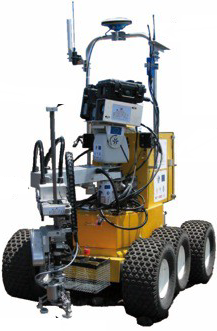
\includegraphics[width=.5\linewidth]{fig_00}}
\def\xxpied{%
\textsf{\xxactivite}%dans le but de déterminer les contraintes géométriques dans les mécanismes\\% afin de valider leurs performances.\\
%Révisions 1 -- 2 -- 3 -- \xxactivite%
}

\def\xxposongletx{2}
\def\xxposonglettext{1.45}
\def\xxposonglety{20}
%\def\xxonglet{Part. 1 -- Ch. 3}


\usepackage{multicol}
\usepackage{siunitx}

\fichetrue
%\fichefalse

\proftrue
\proffalse

\tdtrue
\tdfalse

\courstrue
\coursfalse

\setcounter{secnumdepth}{5}
%---------------------------------------------------------------------------


\begin{document}
%\chapterimage{png/Fond_Cin}
\pagestyle{empty}


%%%%%%%% PAGE DE GARDE COURS
\ifcours
\begin{tikzpicture}[remember picture,overlay]
\node at (current page.north west)
{\begin{tikzpicture}[remember picture,overlay]
\node[anchor=north west,inner sep=0pt] at (0,0) {\includegraphics[width=\paperwidth]{\thechapterimage}};
\draw[anchor=west] (-2cm,-8cm) node [line width=2pt,rounded corners=15pt,draw=ocre,fill=white,fill opacity=0.6,inner sep=40pt]{\strut\makebox[22cm]{}};
\draw[anchor=west] (1cm,-8cm) node {\huge\sffamily\bfseries\color{black} %
\begin{minipage}{1cm}
\rotatebox{90}{\LARGE\sffamily\textsc{\color{ocre}\textbf{\xxnumpartie}}}
\end{minipage} \hfill
\begin{minipage}[c]{14cm}
\begin{titrepartie}
\begin{flushright}
\renewcommand{\baselinestretch}{1.1} 
\Large\sffamily\textsc{\textbf{\xxpartie}}
\renewcommand{\baselinestretch}{1} 
\end{flushright}
\end{titrepartie}
\end{minipage} \hfill
\begin{minipage}[c]{3.5cm}
{\large\sffamily\textsc{\textbf{\color{ocre} \discipline}}}
\end{minipage} 
 };
\end{tikzpicture}};
\end{tikzpicture}


\begin{tikzpicture}[overlay]
\node[shape=rectangle, 
      rounded corners = .25 cm,
	  draw= ocre,
	  line width=2pt, 
	  fill = ocre!10,
	  minimum width  = 2.5cm,
	  minimum height = 3cm,] at (18cm,0) {};
\node at (17.7cm,0) {\rotatebox{90}{\textbf{\Large\color{ocre}{\classe}}}};
%{};
\end{tikzpicture}

\vspace{3.5cm}

\begin{tikzpicture}[remember picture,overlay]
\draw[anchor=west] (-2cm,-6cm) node {\huge\sffamily\bfseries\color{black} %
\begin{minipage}{2cm}
\begin{center}
\LARGE\sffamily\textsc{\color{ocre}\textbf{\xxactivite}}
\end{center}
\end{minipage} \hfill
\begin{minipage}[c]{15cm}
\begin{titrechapitre}
\renewcommand{\baselinestretch}{1.1} 
\Large\sffamily\textsc{\textbf{\xxnumchapitre}}

\Large\sffamily\textsc{\textbf{\xxchapitre}}
\vspace{.5cm}

\renewcommand{\baselinestretch}{1} 
\normalsize\normalfont
\xxcompetences
\end{titrechapitre}
\end{minipage}  };
\end{tikzpicture}
\vfill

\begin{flushright}
\begin{minipage}[c]{.3\linewidth}
\begin{center}
\xxfigures
\end{center}
\end{minipage}\hfill
\begin{minipage}[c]{.6\linewidth}
\startcontents
\printcontents{}{1}{}
\end{minipage}
\end{flushright}

\begin{tikzpicture}[remember picture,overlay]
\draw[anchor=west] (4.5cm,-.7cm) node {
\begin{minipage}[c]{.2\linewidth}
\begin{flushright}
\includegraphics[width=2cm]{png/logoCC}
\end{flushright}
\end{minipage}
\begin{minipage}[c]{.2\linewidth}
\textsl{\xxauteur} \\
\textsl{\classe}
\end{minipage}
 };
\end{tikzpicture}
\newpage
\pagestyle{fancy}

\newpage
\pagestyle{fancy}

\else
\fi


%%%%%%%% PAGE DE GARDE TD
\iftd
%\begin{tikzpicture}[remember picture,overlay]
%\node at (current page.north west)
%{\begin{tikzpicture}[remember picture,overlay]
%\draw[anchor=west] (-2cm,-3.25cm) node [line width=2pt,rounded corners=15pt,draw=ocre,fill=white,fill opacity=0.6,inner sep=40pt]{\strut\makebox[22cm]{}};
%\draw[anchor=west] (1cm,-3.25cm) node {\huge\sffamily\bfseries\color{black} %
%\begin{minipage}{1cm}
%\rotatebox{90}{\LARGE\sffamily\textsc{\color{ocre}\textbf{\xxnumpartie}}}
%\end{minipage} \hfill
%\begin{minipage}[c]{13.5cm}
%\begin{titrepartie}
%\begin{flushright}
%\renewcommand{\baselinestretch}{1.1} 
%\Large\sffamily\textsc{\textbf{\xxpartie}}
%\renewcommand{\baselinestretch}{1} 
%\end{flushright}
%\end{titrepartie}
%\end{minipage} \hfill
%\begin{minipage}[c]{3.5cm}
%{\large\sffamily\textsc{\textbf{\color{ocre} \discipline}}}
%\end{minipage} 
% };
%\end{tikzpicture}};
%\end{tikzpicture}

%%%%%%%%%% PAGE DE GARDE TD %%%%%%%%%%%%%%%
%\begin{tikzpicture}[overlay]
%\node[shape=rectangle, 
%      rounded corners = .25 cm,
%	  draw= ocre,
%	  line width=2pt, 
%	  fill = ocre!10,
%	  minimum width  = 2.5cm,
%	  minimum height = 2.5cm,] at (18.5cm,0) {};
%\node at (17.7cm,0) {\rotatebox{90}{\textbf{\Large\color{ocre}{\classe}}}};
%%{};
%\end{tikzpicture}

% PARTIE ET CHAPITRE
%\begin{tikzpicture}[remember picture,overlay]
%\draw[anchor=west] (-1cm,-2.1cm) node {\large\sffamily\bfseries\color{black} %
%\begin{minipage}[c]{15cm}
%\begin{flushleft}
%\xxnumchapitre \\
%\xxchapitre
%\end{flushleft}
%\end{minipage}  };
%\end{tikzpicture}

% Bandeau titre exo
\begin{tikzpicture}[remember picture,overlay]
\draw[anchor=west] (-2cm,-4cm) node {\huge\sffamily\bfseries\color{black} %
\begin{minipage}{5cm}
\begin{center}
\LARGE\sffamily\color{ocre}\textbf{\textsc{\xxactivite}}

\begin{center}
\xxfigures
\end{center}

\end{center}
\end{minipage} \hfill
\begin{minipage}[c]{12cm}
\begin{titrechapitre}
\renewcommand{\baselinestretch}{1.1} 
\large\sffamily\textbf{\textsc{\xxtitreexo}}

\small\sffamily{\textbf{\textit{\color{black!70}\xxsourceexo}}}
\vspace{.5cm}

\renewcommand{\baselinestretch}{1} 
\normalsize\normalfont
\xxcompetences
\end{titrechapitre}
\end{minipage}  };
\end{tikzpicture}

\else
\fi


%%%%%%%% PAGE DE GARDE FICHE
\iffiche
\begin{tikzpicture}[remember picture,overlay]
\node at (current page.north west)
{\begin{tikzpicture}[remember picture,overlay]
\draw[anchor=west] (-2cm,-3.25cm) node [line width=2pt,rounded corners=15pt,draw=ocre,fill=white,fill opacity=0.6,inner sep=40pt]{\strut\makebox[22cm]{}};
\draw[anchor=west] (1cm,-3.25cm) node {\huge\sffamily\bfseries\color{black} %
\begin{minipage}{1cm}
\rotatebox{90}{\LARGE\sffamily\textsc{\color{ocre}\textbf{\xxnumpartie}}}
\end{minipage} \hfill
\begin{minipage}[c]{14cm}
\begin{titrepartie}
\begin{flushright}
\renewcommand{\baselinestretch}{1.1} 
\large\sffamily\textsc{\textbf{\xxpartie} \\} 

\vspace{.2cm}

\normalsize\sffamily\textsc{\textbf{\xxnumchapitre -- \xxchapitre}}
\renewcommand{\baselinestretch}{1} 
\end{flushright}
\end{titrepartie}
\end{minipage} \hfill
\begin{minipage}[c]{3.5cm}
{\large\sffamily\textsc{\textbf{\color{ocre} \discipline}}}
\end{minipage} 
 };
\end{tikzpicture}};
\end{tikzpicture}


\begin{tikzpicture}[overlay]
\node[shape=rectangle, 
      rounded corners = .25 cm,
	  draw= ocre,
	  line width=2pt, 
	  fill = ocre!10,
	  minimum width  = 2.5cm,
	  minimum height = 2.5cm,] at (18.5cm,0.cm) {};
%	  minimum height = 2.5cm,] at (18.5cm,0cm) {};
\node at (17.7cm,0cm) {\rotatebox{90}{\textsf{\textbf{\large\color{ocre}{\classe}}}}};
%{};
\end{tikzpicture}



\else
\fi



%\vspace{4.5cm}
\pagestyle{fancy}
\thispagestyle{plain}


\def\columnseprulecolor{\color{ocre}}
\setlength{\columnseprule}{0.4pt} 


\begin{tikzpicture}[remember picture,overlay]
\draw[anchor=west] (-2cm,-4cm) node {\huge\sffamily\bfseries\color{black} %
\begin{minipage}{5cm}
\begin{center}
\LARGE\sffamily\color{ocre}\textbf{\textsc{\xxactivite}}

\begin{center}
\xxfigures
\end{center}

\end{center}
\end{minipage} \hfill
\begin{minipage}[c]{12cm}
\begin{titrechapitre}
\renewcommand{\baselinestretch}{1.1} 
\large\sffamily\textbf{\textsc{\xxtitreexo}}

\small\sffamily{\textbf{\textit{\color{black!70}\xxsourceexo}}}
\vspace{.5cm}

\renewcommand{\baselinestretch}{1} 
\normalsize\normalfont
%\xxcompetences
\end{titrechapitre}
\end{minipage}};
\end{tikzpicture}

\vspace{6cm}


\textbf{Commentaires généraux}

\begin{itemize}
\item Il faut être plus rigoureux sur les énoncés des théorèmes (théorème du moment dynamique $\neq$ théorème de lé résultante dynamqiue $\neq$ PFD).
\item Revoir le calcul de l'énergie cinétique d'une roue. 
\item Revoir le calcul de la puissance dans une liaison ponctuelle avec frottement et RSG. 
\item Il faut être plus rigoureux sur les notations en énergétiques ($\pext{1}{2}{0}$).
\item PLEASE : je ne veux plus lire que $FTBF=FTBO/(1+FTBO)$ c'est une horreur inqualifiable quand le retour n'est pas unitaire. 
\item L'avantage du correcteur PI est avant tout d'ajouter une classe au système et donc de réduire les erreurs (statique, en vitesse, en accélération ...). Il peut ensuite stabiliser le système ou le désabiliser s'il est mal réglé...
\end{itemize}

Extrait du rapport CCMP -- PSI -- 2021
\begin{itemize}
\item Q1 - Question classique d’étude d’une loi de vitesse en trapèze. Il faut veiller à répondre correctement
à la question, en donnant les expressions littérales demandées. Le résultat seul ne suffit pas, et les
applications numériques doivent être correctement effectuées.
\item Q2 - Question souvent bien traitée, malgré une erreur de signe fréquente liée à une mauvaise analyse
du paramétrage. Trop d’erreurs sur les calculs simples d’énergie cinétique (POUR LA ROUE, OUBLI DE L'ENRGIE CINETIQUE DE ROTATION OU DE TRANSLATION).
\item Q3 - Il était demandé un bilan de puissance nécessaire à l’application du Théorème de l’Energie
Cinétique (Q4). Cette question a été extrêmement mal traitée. Il faut absolument identifier clairement
le système étudié, et lister proprement les actions mécaniques intérieures et extérieures. Le roulement
sans glissement a posé beaucoup de problèmes dans l’expression des puissances extérieures. Ce genre
de question ne peut être traité correctement qu’avec rigueur. 
\item Q4 - Question mal traitée, du fait des problèmes rencontrés en Q3. Attention à bien donner le résultat
sous la forme demandée dans l’énoncé.
\item Q5 - Question destinée à préparer la Q6. Beaucoup d’erreurs ont été commises suite à un mauvais
Bilan des Actions Mécaniques Extérieures s’exerçant sur la roue. Identifier un cas simple permet de
s’affranchir de calculs inutilement compliqués.
\item Q6 - Application du Théorème du Moment Dynamique à un solide unique. Cette question a été bien
réussie quand la Q5 l’a été également. Trop de réponses sont données sans se soucier de la forme
demandée dans la question. C’est dommage de perdre des points pour cela alors que la méthode est
bonne.
\item Q7 - Cette question interrogeait le candidat sur sa capacité à choisir la méthode de résolution du
problème posé. Choisir la bonne équation à écrire permet d’optimiser la résolution du problème.
Cependant, même lorsque la méthode choisie était la bonne, les calculs menés pour déterminer le
moment dynamique n’ont que trop rarement abouti.
\item Q8 - Comme pour Q7, cette question évaluait plutôt la capacité du candidat à définir une démarche
de résolution. Aucun calcul n’était demandé, mais on peut noter qu’une fois encore, le Bilan des
Actions Mécaniques Extérieures a été trop souvent négligé. Le jury souhaite mettre l’accent sur le
fait qu’annoncer un Bilan des Actions Mécaniques Extérieures et un théorème sans avoir au préalable
indiqué l’isolement n’a pas de sens ! Le jury a donc sanctionné les candidats qui n’auraient pas indiqué
l’isolement.
\item Q9 - Cette question permettait de relier les calculs menés de Q5 à Q8 à la problématique de la partie
1. En utilisant le modèle de Coulomb, visiblement mal maitrisé par les candidats, il suffisait de relier le
facteur de frottement aux actions mécaniques déterminées précédemment. Attention à ne pas oublier
les valeurs absolues dans le calcul lorsqu’on établit le facteur de frottement nécessaire.
\item Q10 - Les valeurs étant données, le candidat devait simplement prendre en considération la simplification
du modèle (passage de 2 à 4 roues) et le coefficient de sécurité pour définir le facteur de frottement
minimal à prendre en compte pour choisir le couple de matériaux en jeu. Une fois encore, trop de
réponses ont été incomplètes ou incorrectes, du fait d’une mauvaise compréhension des phénomènes et
d’une mauvaise lecture de l’énoncé.
\item  Q11 - Dans cette question, il n’était pas
demandé de mener intégralement les calculs. Une analyse des mobilités permettait notamment de
répondre à la question de manière rapide et efficace. Les candidats qui se sont lancés dans des calculs
ont perdu beaucoup de temps. Quoi qu’il en soit, la démarche devait être expliquée, quelle que soit
la méthode choisie. A noter que la réponse était immédiate quand on pensait à écrire directement
les torseurs des liaisons sphère/plan en L et L’ (la forme des torseurs se conserve en tout point de la
normale au contact).
\item Q12 - Mêmes remarques que pour Q11. Pour ce qui est de la conclusion, trop de candidats utilisent
l’hyperstatisme comme réponse magique pour justifier le choix d’architecture, sans maîtriser les concepts
utilisés. Il ne s’agissait ici que d’un choix fonctionnel.
\item Q13 - Beaucoup d’erreurs dans l’inventaire des actions mécaniques extérieures, qui aboutissent à une
mauvaise utilisation du Théorème de la Résultante Statique, alors qu’un simple Théorème du Moment
Statique permettait de résoudre ce problème très facilement. Trop de candidats proposent une réponse
sans recul, notamment en laissant de côté les problématiques de signe et leur interprétation physique.
\item Q14 - Trop d’erreurs sur le calcul simple de volume. Là aussi, beaucoup de problèmes de signes qui
aboutissent à des non-sens physiques.
\item Q15 - Cette question a été plutôt réussie par les candidats, surtout sur l’analyse de l’intérêt du
dispositif de contrepoids. En revanche, l’analyse de l’influence de la position du poids d’ancrage a
souvent été mal menée, de nombreux candidats se contentant de répondre sans argumenter.
\item Q16 - De nombreux résultats fantaisistes ont été proposés par les candidats pour cette étude de théorie
des mécanismes, démontrant une fois encore que la notion d’hyperstatisme est mal maîtrisée. Il est
important d’être rigoureux dans la méthode pour aboutir à un résultat correct. De nombreux candidats
se sont par exemple trompés dans l’analyse des mobilités (les correcteurs ont parfois eu l’impression que
les mobilités étaient une variable d’ajustement pour aboutir miraculeusement à un modèle isostatique).
Dire simplement sans argumenter que le système est isostatique en guise de conclusion n’est pas
suffisant.
\item Q17 - Malgré les indices proposés par le sujet, peu de candidats ont pensé à appliquer le Principe
Fondamental de la Dynamique pour cette question, qui a finalement été peu abordée. Là encore,
impossible de s’en sortir sans un Bilan des Actions Mécaniques Extérieures rigoureux.
\item Q18 - Cette question a été bien traitée par les candidats qui ont bien traité Q17. Dans ce cas, cette
question restait très abordable.
\item Q19 - Trop de candidats se sont focalisés sur la démonstration (plus ou moins approximative) que le
torseur proposé était un glisseur, alors que l’esprit de la question était d’étudier l’équilibre de la barre
soumise à 2 glisseurs, pour en déterminer la droite support.
\item Q20 - L’objectif de cette question était de préparer le Bilan des Actions Mécaniques Extérieures pour
la Q21. Elle a très peu été abordée par les candidats alors qu’elle était le simple prolongement de la
question précédente. Le jury rappelle au candidat la nécessité d’écrire les torseurs avec rigueur (point,
base, etc. . . ).
\item Q21 - Cette question, bien qu’assez calculatoire, ne présentait pas d’autre difficulté majeure. En effet,
il suffisait d’isoler un seul solide et d’exprimer tous les torseurs au même point. Les calculs ont été
dans l’ensemble plutôt bien menés lorsque cette partie du sujet a été traitée par les candidats.
\item Q22 - Les expressions trouvées en Q21 faisant apparaître la grandeur λ, il fallait proposer un dispositif
permettant de connaître cette grandeur en temps réel. Le diagramme de définition de blocs en annexe
5 donnait la réponse. A défaut, toute solution technologique crédible et correctement définie a été
acceptée par le jury.
\item Q23 - Cette première question d’asservissement demandait aux candidats d’analyser un schéma-blocs
et d’en déduire le modèle de 3 gains. En particulier, les candidats étaient invités à bien faire apparaitre
les unités et devaient maitriser une condition « de bon fonctionnement ».
\item Q24 - Cette question, destinée à préparer la question Q25, demandait de calculer 2 fonctions de
transfert d’un asservissement, l’une vis-à-vis de la seule consigne et l’autre vis-à-vis de la seule
perturbation. C’est dommage que certains candidats n’aient pas pris le temps de bien lire les définitions
des grandeurs et se soient trompés de signe. Une question pratiquement toujours traitée avec beaucoup
de réussite.
\item Q25 - Une question bien traitée en général quand la question Q24 l’avait été correctement.
\item Q26 - Question classique demandant de calculer l’erreur statique et l’erreur de trainage, en utilisant
le théorème de la valeur finale. La FTBO étant de classe 1, il était possible de répondre sans calcul.
Attention à la manipulation des inégalités dans la détermination de la condition limite sur C.
\item Q27 - Une question classique qui évaluait la capacité des candidats à déterminer une valeur limite du
gain du correcteur proportionnel-Intégral à partir d’un diagramme de Bode de la FTBO afin de satisfaire
les marges de stabilité. La méthode graphique était la plus efficace, mais une résolution analytique
était possible. Le jury trouve dommage que cette compétence classique n’ait pas été suffisamment bien
maîtrisée.
\item Q28 - Question bien traitée lorsque Q26 et Q27 l’ont été aussi. Dans le cas contraire, il était impossible
de conclure correctement.
\item Q29 - Question assez facile portant sur la manipulation de la fonction de transfert du correcteur ;
abordée correctement par une grande majorité des candidats.
\item Q30 - Mêmes remarques que pour la question 26.
\item Q31 - Le tracé demandé était relativement classique. Le jury a constaté beaucoup trop d’erreurs pour
une question d’une difficulté très relative.
\item Q32 - Cette question demandait au candidat de relever 3 valeurs caractéristiques sur les courbes,
et d’en déduire si oui ou non l’exigence 1.2 était satisfaite. Les relevés sont la plupart du temps très
approximatifs et l’analyse de la satisfaction du cahier des charges manque de rigueur. Il fallait passer
en revue les 4 exigences et comparer les relevés aux valeurs seuil définies dans le cahier des charges. Il
ne suffit pas d’affirmer sans preuve qu’une exigence est satisfaite !
\item Q33 - Question classique destinée à mettre en évidence les limites d’un modèle linéaire. Beaucoup
trop de candidats confondent courbes expérimentales et simulation.
\end{itemize}

Extrait du rapport CCINP -- PSI -- 2021
\begin{itemize}
\item Q1. Question globalement bien traitée. Quelques candidats réussissent tout de même à écrire des formules
non homogènes.
\item Q3. Question assez bien traitée. Il est vivement recommandé d’expliquer un résultat littéral avant de faire
l’application numérique.
\item Q5. Question assez bien traitée, même si la constante de temps du modèle du 1er ordre n’est pas toujours bien
identifiée.
\item Q6. Question moyennement bien traitée. La solution temporelle était donnée à la question précédente, il n’y
avait pourtant pas de difficultés. Tous les candidats ne connaissent pas la réponse d’un système du
1
er ordre suite à une entrée de type rampe.
\item Q7. Question bien traitée dans l’ensemble par les candidats. Il fallait exprimer les résultats sous forme
canonique comme la question le stipulait.
\item Q8. Question globalement bien traitée. La relation entre les gains de l’adaptateur, du codeur et du
transmetteur a posé beaucoup de difficultés aux candidats.
\item Q9. Question qui a donné lieu à la découverte de nouveaux noms de correcteurs… Quand le terme
proportionnel-intégral a été fourni, la justification a trop souvent été d’améliorer la stabilité !
\item Q10. Question assez peu traitée par les candidats. Pour ceux qui l’ont faite, il y a toujours des confusions
entre la constante de temps de la fonction de transfert en boucle fermée et le temps de réponse à 5 %.
\item Q11. Question où le seuil a été majoritairement donné comme réponse. Toutefois beaucoup de copies ont
parlé d’hystérésis…
\item Q12. Question souvent très mal traitée. La masse équivalente a souvent été justifiée en donnant la masse de
l’ensemble sans se référer à l’énergie cinétique de l’ensemble. Les autres grandeurs ont rarement été
cherchées.
\item Q13. et Q14. Questions assez bien traitées par le peu de candidats qui les ont abordées.
\item Q15. Question globalement bien traitée. On notera quelques erreurs de signes tout de même.
\item Q16. Question assez bien traitée par les candidats ayant traité la question précédente correctement.
\item Q19. Question très mal traitée. On note le manque de culture technologique sans doute dû aux divers
confinements.
\item Q20. Très peu de candidats arrivent à expliquer pourquoi le pot reste parallèle au sol en phase d’élévation et
parlent du parallélogramme déformable.
\item Q21. Un nombre beaucoup trop important de candidats annonce une mobilité nulle ou encore différente de 1.
\item Q22. Question où l’on a vu énormément de solutions fausses modifiant la mobilité utile et trop rarement une
solution correcte. Certains candidats ont travaillé sur le système de la question précédente.
\item Q23. Les candidats ayant pris soin de bien écrire le bilan des actions mécaniques et connaissant les lois de
Coulomb ont réussi cette question assez rarement traitée.
\item Q24. Question ouverte difficile qui a été assez mal traitée quand elle a été tentée. Beaucoup de candidats
arrivent à trouver le résultat en appliquant le théorème du moment statique sur le pot !
\item Q25. Question souvent bien traitée. Le bon sens a néanmoins manqué dans quelques copies.
\item Q28. Question assez mal traitée. Beaucoup de candidats utilisent des théorèmes de statique ; le PFD tout
court. On retrouve assez souvent la formulation « Théorème de la résultante dynamique au point G en
projection sur… », il serait bon de ne pas écrire « au point G » même si les correcteurs comprennent
pourquoi ils le font.
\item Q30. Question moyennement bien traitée du fait des applications numériques un peu longues et la fin du
sujet approchant.
\item Q31. Question mal traitée.
\item Q32. L’ordre des états a été rarement mis dans le bon ordre.
\item Q33. Les transitions ont été assez bien complétées (par rapport à l’ordre que les candidats ont donné aux
états à la question précédente). Seule l’incrémentation du compteur a été rarement réalisée.
\end{itemize}
%
%\textbf{Remarques}
%\begin{itemize}
%\item Question 1 : lors de la réalisation du schéma cinématique, l'algnement des liaisons doit être respecté, comme c'est le cas dans le mécanisme réel. Les couleurs des pièces participant aux la liaison doivent être respectées (une liaisons met deux pièces en relation, il faut respecter la couleur de l'axe et du corps de la liaison \textit{etc}.). 
%\item Question 2 : beaucoup d'entre vous ont du mal à identifier quelles sont les liaisons en parallèle et en série dans le mécanisme donné. Par ailleurs, intuiter une liaison équivalente ne suffit pas. Il faut justifier par le calcul. 
%Enfin, dans le cas des liaisons hélicoïdales et pivot qui étaient en série. On trouve une liaison avec une composante en $\omega_x$ et en $V_x$ parmi lesquelles il y a 3 inconnues indépendantes. La liaison équivalente est donc une liaison pivot glissant.
%\item Question 3 : deux raisonnements élémentaires de cinématiques non maîtrisés par la plupart d'entre vous : décomposition du vecteur vitesse, utilisation de la formule de Varignon.
%\item Question 5, il s'agissait de projeter le vecteur $\vect{n}$ dnas la base $\base{x_0}{y_0}{z_0}$. Beaucoup y parviennent sans erreur.
%\item Question 6 et 7 : calcul de la norme d'un vecteur qui n'aurait pas du poser de problème... puis application numérique...
%\item Question 8 : la résolution du capteur n'aurait pas dû poser de problème (il fallait aussi prendre en compte l'existence d'un réducteur).
%\item Question 9 : attention, il s'agissait d'isoler l'ensemble motorisé. Cet ensemble était situé entre 2 rotules qui sont des glisseurs... le PFS indique directement que l'action est dans la direction joignant le centre des rotules.
%\item Question 10 : question délicate sur le papier ... mais qui ne se passe pas si mal en écrivant la démarche méthodiquement. 
%\item Question 11 : il s'agissait de LA QUESTION d'hyperstatisme... que peu ont vu.
%\item Question 12 : question sans vraiment de diffuculté. 
%\item Question 13 : bien traitée par la plupart.
%\item Question 14 à 16 : questions qui n'auraient pas dû poser de difficulté. 
%\item Question 17 à 20 : questions difficiles. Beaucoup d'entre vous les ont sauter et on eu raison... mais n'ont pas pris suffisamment de points ailleurs...
%\item Question 21 : il faut savoir tracer le diagramme de Bode d'un retard. Le module de $e^{-Tj\omega}$ est 1. La phase est $-T\omega$ (en rad).
%\item Question 22 : beaucoup d'aspects dans cette question, mais il faut tout traiter avec rigueur : 
%\begin{itemize}
%\item déterminer des marges avec et sans retard;
%\item exprimer les conditions de stablité;
%\item tracer le Bode d'un correcteur.
%\end{itemize}
%Même si cette question peut paraître difficile vous devez être capables de traiter tous les aspects de la question.
%\item Question 23 : TB.
%\item Question 24 : beaucoup d'erreurs dans le calcul du module et de la phase d'une fonction de transfert. \textbf{Il faut s'entrainer abolument !!}
%\item Question 25 et 26 : beaucoup d'erreurs sur ces questions. Ce n'est pas normal. \textbf{Il faut s'entrainer abolument !!}
%\item Question 27 : cette question doit être absolument traitée. Il faut déterminer des valeurs numériques sur des courbes et valider (ou non) le cahier des charges. \textbf{A faire !}
%\end{itemize}
%



\begin{minipage}[c]{.45\linewidth} 
\Large \textbf{\textsf{NOM00 Prenom00}} 
 
 \normalsize Note harmonisée 8.63/20 
 
Rang 3
 
Moyenne classe harmonisée 7.13/20 
 
Moyenne question traitées 8.63/20 
 
Rang question traitées 10 
 
Commentaires : 
Comment1 
\end{minipage}\hfill 
\begin{minipage}[c]{.45\linewidth}  
\begin{center}
\includegraphics[width=.8\linewidth]{../histo.pdf} 
\end{center}
\end{minipage}
\footnotesize 
\begin{center} 
\begin{tabular}{|c|c|m{1cm}|c||c|c|m{1cm}|c||c|c|m{1cm}|c||c|c|m{1cm}|c|} 
\hline \textbf{Qu} & \textbf{Coef} & \textbf{Comp} & \textbf{/5} & \textbf{Qu} & \textbf{Coef} & \textbf{Comp} & \textbf{/5} & \textbf{Qu} & \textbf{Coef} & \textbf{Comp} & \textbf{/5} & \textbf{Qu} & \textbf{Coef} & \textbf{Comp} & \textbf{/5} \\ 
\hline 
\hline 
Q1 & 1 & A1-01 & 5 & Q1 & 1 & A1-02 & 4 & Q2 & 1 & A1-03 & 3 & Q2 & 1 & A1-04 & 2 \\ \hline 
 
Q3 & 1 & A1-05 & 1 & Q4 & 1 & A2-01 & 0 & Q5 & 1 & A2-02 & 5 & Q6 & 2 & A2-03 & 4 \\ \hline 
 
Q7 & 2 & A3-01 & 3 & Q8 & 2 & A3-02 & 2 & Q9 & 3 & A3-03 & 1 &  &  &  &  \\ \hline 
 
\end{tabular} 
\end{center} 
\normalsize 
 


%\section{A -- Analyser}  
\subsection{A1 -- Analyser le besoin et les exigences}  
\subsubsection*{A1-01 -- Décrire le besoin et les exigences.}  
\begin{center} 
\includegraphics{A1-01.pdf} 
\end{center} 
\subsubsection*{A1-02 -- Traduire un besoin fonctionnel en exigences.}  
\begin{center} 
\includegraphics{A1-02.pdf} 
\end{center} 
\subsubsection*{A1-03 -- Définir les domaines d’application et les critères technico-économiques et environnementaux.}  
\begin{center} 
\includegraphics{A1-03.pdf} 
\end{center} 
\subsubsection*{A1-04 -- Qualifier et quantifier les exigences.}  
\begin{center} 
\includegraphics{A1-04.pdf} 
\end{center} 
\subsubsection*{A1-05 -- Évaluer l’impact environnemental et sociétal.}  
\begin{center} 
\includegraphics{A1-05.pdf} 
\end{center} 
\subsection{A2 -- Définir les frontières de l'analyse}  
\subsubsection*{A2-01 -- Isoler un système et justifier l’isolement.}  
\begin{center} 
\includegraphics{A2-01.pdf} 
\end{center} 
\subsubsection*{A2-02 -- Définir les éléments influents du milieu extérieur. }  
\begin{center} 
\includegraphics{A2-02.pdf} 
\end{center} 
\subsubsection*{A2-03 -- Identifier la nature des flux échangés traversant la frontière d’étude.}  
\begin{center} 
\includegraphics{A2-03.pdf} 
\end{center} 
\subsection{A3 -- Analyser l'organisation fonctionnelle et structurelle}  
\subsubsection*{A3-01 -- Associer les fonctions aux constituants.}  
\begin{center} 
\includegraphics{A3-01.pdf} 
\end{center} 
\subsubsection*{A3-02 -- Justifier le choix des constituants dédiés aux fonctions d’un système.}  
\begin{center} 
\includegraphics{A3-02.pdf} 
\end{center} 
\subsubsection*{A3-03 -- Identifier et décrire les chaines fonctionnelles du système.}  
\begin{center} 
\includegraphics{A3-03.pdf} 
\end{center} 
\subsubsection*{A3-04 -- Identifier et décrire les liens entre les chaines fonctionnelles.}  
\subsubsection*{A3-05 -- Caractériser un constituant de la chaine de puissance.}  
\subsubsection*{A3-06 -- Caractériser un constituant de la chaine d’information.}  
\subsubsection*{A3-07 -- Analyser un algorithme. }  
\subsubsection*{A3-08 -- Analyser les principes d'intelligence artificielle. }  
\subsubsection*{A3-09 -- Interpréter tout ou partie de l’évolution temporelle d’un système séquentiel.}  
\subsubsection*{A3-10 -- Identifier la structure d'un système asservi.}  
\subsection{A4 -- Analyser les performances et les écarts}  
\subsubsection*{A4-01 -- Extraire un indicateur de performance pertinent à partir du cahier des charges ou de résultats issus de l'expérimentation ou de la simulation.}  
\subsubsection*{A4-02 -- Caractériser les écarts entre les performances.}  
\subsubsection*{A4-03 -- Interpréter et vérifier la cohérence des résultats obtenus expérimentalement, analytiquement ou numériquement. }  
\subsubsection*{A4-04 -- Rechercher et proposer des causes aux écarts constatés.}  
\section{B -- Modéliser}  
\subsection{B1 -- Choisir les grandeurs physiques et les caractériser}  
\subsubsection*{B1-01 -- Identifier les performances à prévoir ou à évaluer.}  
\subsubsection*{B1-02 -- Identifier les grandeurs d'entrée et de sortie d’un modèle.}  
\subsubsection*{B1-03 -- Identifier les paramètres d’un modèle.}  
\subsubsection*{B1-04 -- Identifier et justifier les hypothèses nécessaires à la modélisation.}  
\subsection{B2 -- Proposer un modèle de connaissance et de comportement}  
\subsubsection*{B2-01 -- Choisir un modèle adapté aux performances à prévoir ou à évaluer.}  
\subsubsection*{B2-02 -- Compléter un modèle multiphysique.}  
\subsubsection*{B2-03 -- Associer un modèle aux composants des chaines fonctionnelles.}  
\subsubsection*{B2-04 -- Établir un modèle de connaissance par des fonctions de transfert.}  
\subsubsection*{B2-05 -- Modéliser le signal d'entrée.}  
\subsubsection*{B2-06 -- Établir un modèle de comportement à partir d'une réponse temporelle ou fréquentielle. }  
\subsubsection*{B2-07 -- Modéliser un système par schéma-blocs. }  
\subsubsection*{B2-08 -- Simplifier un modèle.}  
\subsubsection*{B2-09 -- Modéliser un correcteur numérique. }  
\subsubsection*{B2-10 -- Déterminer les caractéristiques d'un solide ou d'un ensemble de solides indéformables.}  
\subsubsection*{B2-11 -- Proposer une modélisation des liaisons avec leurs caractéristiques géométriques.}  
\subsubsection*{B2-12 -- Proposer un modèle cinématique à partir d'un système réel ou d'une maquette numérique.}  
\subsubsection*{B2-13 -- Modéliser la cinématique d'un ensemble de solides.}  
\subsubsection*{B2-14 -- Modéliser une action mécanique.}  
\subsubsection*{B2-15 -- Simplifier un modèle de mécanisme.}  
\subsubsection*{B2-16 -- Modifier un modèle pour le rendre isostatique.}  
\subsubsection*{B2-17 -- Décrire le comportement d'un système séquentiel.}  
\subsection{B3 -- Valider un modèle}  
\subsubsection*{B3-01 -- Vérifier la cohérence du modèle choisi en confrontant les résultats analytiques et/ou numériques aux résultats expérimentaux.}  
\subsubsection*{B3-02 -- Préciser les limites de validité d'un modèle.}  
\subsubsection*{B3-03 -- Modifier les paramètres et enrichir le modèle pour minimiser l’écart entre les résultats analytiques et/ou numériques et les résultats expérimentaux.}  
\section{C -- Résoudre}  
\subsection{C1 -- Proposer une démarche de résolution}  
\subsubsection*{C1-01 -- Proposer une démarche permettant d'évaluer les performances des systèmes asservis.}  
\subsubsection*{C1-02 -- Proposer une démarche de réglage d'un correcteur.}  
\subsubsection*{C1-03 -- Choisir une démarche de résolution d’un problème d'ingénierie numérique ou d'intelligence artificielle. }  
\subsubsection*{C1-04 -- Proposer une démarche permettant d'obtenir une loi entrée-sortie géométrique. }  
\subsubsection*{C1-05 -- Proposer une démarche permettant la détermination d’une action mécanique inconnue ou d'une loi de mouvement.}  
\subsection{C2 -- Mettre en œuvre une démarche de résolution analytique}  
\subsubsection*{C2-01 -- Déterminer la réponse temporelle.}  
\subsubsection*{C2-02 -- Déterminer la réponse fréquentielle. }  
\subsubsection*{C2-03 -- Déterminer les performances d'un système asservi.}  
\subsubsection*{C2-04 -- Mettre en œuvre une démarche de réglage d’un correcteur.}  
\subsubsection*{C2-05 -- Caractériser le mouvement d’un repère par rapport à un autre repère.}  
\subsubsection*{C2-06 -- Déterminer les relations entre les grandeurs géométriques ou cinématiques. }  
\subsubsection*{C2-07 -- Déterminer les actions mécaniques en statique.}  
\subsubsection*{C2-08 -- Déterminer les actions mécaniques en dynamique dans le cas où le mouvement est imposé.}  
\subsubsection*{C2-09 -- Déterminer la loi de mouvement dans le cas où les efforts extérieurs sont connus.}  
\subsection{C3 -- Mettre en œuvre une démarche de résolution numérique}  
\subsubsection*{C3-01 -- Mener une simulation numérique. }  
\subsubsection*{C3-02 -- Résoudre numériquement une équation ou un système d'équations. }  
\subsubsection*{C3-03 -- Résoudre un problème en utilisant une solution d'intelligence artificielle. }  
\section{D -- Expérimenter}  
\subsection{D1 -- Mettre en œuvre un système}  
\subsubsection*{D1-01 -- Mettre en œuvre un système en suivant un protocole.}  
\subsubsection*{D1-02 -- Repérer les constituants réalisant les principales fonctions des chaines fonctionnelles.}  
\subsubsection*{D1-03 -- Identifier les grandeurs physiques d’effort et de flux.}  
\subsection{D2 -- Proposer et justifier un protocole expérimental}  
\subsubsection*{D2-01 -- Choisir le protocole en fonction de l'objectif visé.}  
\subsubsection*{D2-02 -- Choisir les configurations matérielles et logicielles du système en fonction de l'objectif visé par l'expérimentation.}  
\subsubsection*{D2-03 -- Choisir les réglages du système en fonction de l'objectif visé par l'expérimentation.}  
\subsubsection*{D2-04 -- Choisir la grandeur physique à mesurer ou justifier son choix.}  
\subsubsection*{D2-05 -- Choisir les entrées à imposer et les sorties pour identifier un modèle de comportement.}  
\subsubsection*{D2-06 -- Justifier le choix d’un capteur ou d’un appareil de mesure vis-à-vis de la grandeur physique à mesurer.}  
\subsection{D3 -- Mettre en œuvre un protocole expérimental}  
\subsubsection*{D3-01 -- Régler les paramètres de fonctionnement d'un système.}  
\subsubsection*{D3-02 -- Mettre en œuvre un appareil de mesure adapté à la caractéristique de la grandeur à mesurer.}  
\subsubsection*{D3-03 -- Effectuer des traitements à partir de données. }  
\subsubsection*{D3-04 -- Identifier les erreurs de mesure.}  
\subsubsection*{D3-05 -- Identifier les erreurs de méthode.}  
\section{E -- Communiquer}  
\subsection{E1 -- Rechercher et traiter des informations}  
\subsubsection*{E1-01 -- Rechercher des informations.}  
\subsubsection*{E1-02 -- Distinguer les différents types de documents et de données en fonction de leurs usages.}  
\subsubsection*{E1-03 -- Vérifier la pertinence des informations (obtention, véracité, fiabilité et précision de l'information).}  
\subsubsection*{E1-04 -- Extraire les informations utiles d’un dossier technique.}  
\subsubsection*{E1-05 -- Lire et décoder un document technique.}  
\subsubsection*{E1-06 -- Trier les informations selon des critères.}  
\subsubsection*{E1-07 -- Effectuer une synthèse des informations disponibles dans un dossier technique.}  
\subsection{E2 -- Produire et échanger de l'information}  
\subsubsection*{E2-01 -- Choisir un outil de communication adapté à l’interlocuteur.}  
\subsubsection*{E2-02 -- Faire preuve d’écoute et confronter des points de vue.}  
\subsubsection*{E2-03 -- Présenter les étapes de son travail.}  
\subsubsection*{E2-04 -- Présenter de manière argumentée une synthèse des résultats.}  
\subsubsection*{E2-05 -- Produire des documents techniques adaptés à l'objectif de la communication. }  
\subsubsection*{E2-06 -- Utiliser un vocabulaire technique, des symboles et des unités adéquats.}  
\section{F -- Concevoir}  
\subsection{F1 -- Concevoir l'architecture d'un système innovant}  
\subsubsection*{F1-01 -- Proposer une architecture fonctionnelle et organique.}  
\subsection{F2 -- Proposer et choisir des solutions techniques}  
\subsubsection*{F2-01 -- Modifier la commande pour faire évoluer le comportement du système. }  


\end{document}
